\documentclass[fr]{../../../eplexercises}

% Change APE en TP

\RequirePackage{titlesec}
\titleformat
{\section} % command
[hang] % shape
{\bfseries\Large} % format
{\thesection} % label
{0.5ex} % sep
{} % before-code


\usepackage{../fitch}
\usepackage{pdfpages}

\newcommand{\true}{\mathrm{true}}
\newcommand{\false}{\mathrm{false}}
\newcommand{\val}{\mathrm{val}}
\newcommand{\VAL}{\mathrm{VAL}}
\newcommand{\decale}{\par\nodecale\hspace*{20pt}\ignorespaces}

\hypertitle{logique-INGI1101}{5}{INGI}{1101}
{Adrien Ballet\and Basile Cassiers\and Maxime Dimidschstein\and Samuel Monroe\and Sébastien Mottet\and Grâce Musuvaho\and Nicolas Vanvyve\and Mathias Novak\and Céline Deknop}
{Peter Van Roy}

% OR
\pgfkeys{
	orGate/.is family,
	orGate,
	x/.initial=0,
	y/.initial=0,
	l/.initial=or,
}
\newcommand\orGateSet[1]{\pgfkeys{orGate, #1}}
\newcommand\orGate[1][]{
	\orGateSet{#1,
    x/.get=\x,
    y/.get=\y,
		l/.get=\l,
  }
	\draw (\x, 1 + \y) to [out=0,in=120] (0.85 + \x, 0.5 + \y);
	\draw (\x, \y) to [out=0,in=250] (0.85 + \x, 0.5 + \y);
	\draw (\x, \y) to [out=60,in=270] (0.2 + \x, 0.5 + \y);
	\draw (\x, 1 + \y) to [out=300,in=90] (0.2 + \x, 0.5 + \y);
	\draw (\x, 0.2 + \y) -- (0.12 + \x, 0.2 + \y);
	\draw (\x, 0.8 + \y) -- (0.12 + \x, 0.8 + \y);
	\draw (0.85 + \x, 0.5 + \y) -- (1 + \x, 0.5 + \y);
	\node at (\x + 0.5, \y + 0.5) {\tiny \textsf{\l}};
}

% NOR
\pgfkeys{
	norGate/.is family,
	norGate,
	x/.initial=0,
	y/.initial=0,
	l/.initial=nor,
}
\newcommand\norGateSet[1]{\pgfkeys{norGate, #1}}
\newcommand\norGate[1][]{
	\norGateSet{#1,
    x/.get=\x,
    y/.get=\y,
		l/.get=\l,
  }
	\draw (\x, 1 + \y) to [out=0,in=120] (0.85 + \x, 0.5 + \y);
	\draw (\x, \y) to [out=0,in=250] (0.85 + \x, 0.5 + \y);
	\draw (\x, \y) to [out=60,in=270] (0.2 + \x, 0.5 + \y);
	\draw (\x, 1 + \y) to [out=300,in=90] (0.2 + \x, 0.5 + \y);
	\draw (\x, 0.2 + \y) -- (0.12 + \x, 0.2 + \y);
	\draw (\x, 0.8 + \y) -- (0.12 + \x, 0.8 + \y);
	\draw (0.85 + \x, 0.5 + \y) -- (1 + \x, 0.5 + \y);
	\draw[fill = white] (0.85 + \x, 0.5 + \y) circle (0.04);
	\node at (\x + 0.5, \y + 0.5) {\tiny \textsf{\l}};
}

% AND
\pgfkeys{
	andGate/.is family,
	andGate,
	x/.initial=0,
	y/.initial=0,
	l/.initial=and,
}
\newcommand\andGateSet[1]{\pgfkeys{andGate, #1}}
\newcommand\andGate[1][]{
	\andGateSet{#1,
    x/.get=\x,
    y/.get=\y,
		l/.get=\l,
  }
	\draw (0.1 + \x, \y) -- (0.1 + \x, 1 + \y);
	\draw (0.1 + \x, \y) -- (0.6 + \x, \y);
	\draw (0.1 + \x, 1 + \y) -- (0.6 + \x, 1 + \y);
	\draw (0.6 + \x, \y) to [out=0, in=270] (0.9 + \x, 0.5 + \y);
	\draw (0.6 + \x, 1 + \y) to [out=0, in=90] (0.9 + \x, 0.5 + \y);
	\draw (\x, 0.2 + \y) -- (0.1 + \x, 0.2 + \y);
	\draw (\x, 0.8 + \y) -- (0.1 + \x, 0.8 + \y);
	\draw (0.9 + \x, 0.5 + \y) -- (1 + \x, 0.5 + \y);
	\node at (\x + 0.5, \y + 0.5) {\tiny \textsf{\l}};
}

% NAND
\pgfkeys{
	nandGate/.is family,
	nandGate,
	x/.initial=0,
	y/.initial=0,
	l/.initial=nand,
}
\newcommand\nandGateSet[1]{\pgfkeys{nandGate, #1}}
\newcommand\nandGate[1][]{
	\nandGateSet{#1,
    x/.get=\x,
    y/.get=\y,
		l/.get=\l,
  }
	\draw (0.1 + \x, \y) -- (0.1 + \x, 1 + \y);
	\draw (0.1 + \x, \y) -- (0.6 + \x, \y);
	\draw (0.1 + \x, 1 + \y) -- (0.6 + \x, 1 + \y);
	\draw (0.6 + \x, \y) to [out=0, in=270] (0.9 + \x, 0.5 + \y);
	\draw (0.6 + \x, 1 + \y) to [out=0, in=90] (0.9 + \x, 0.5 + \y);
	\draw (\x, 0.2 + \y) -- (0.1 + \x, 0.2 + \y);
	\draw (\x, 0.8 + \y) -- (0.1 + \x, 0.8 + \y);
	\draw (0.9 + \x, 0.5 + \y) -- (1 + \x, 0.5 + \y);
	\draw[fill = white] (0.9 + \x, 0.5 + \y) circle (0.04);
	\node at (\x + 0.5, \y + 0.5) {\tiny \textsf{\l}};
}

% NOT
\pgfkeys{
	notGate/.is family,
	notGate,
	x/.initial=0,
	y/.initial=0,
	l/.initial=not,
}
\newcommand\notGateSet[1]{\pgfkeys{notGate, #1}}
\newcommand\notGate[1][]{
	\notGateSet{#1,
    x/.get=\x,
    y/.get=\y,
		l/.get=\l,
  }
	\draw (0.1 + \x, \y) -- (0.1 + \x, 1 + \y);
	\draw (0.1 + \x, \y) -- (0.9 + \x, 0.5 + \y);
	\draw (0.1 + \x, 1 + \y) -- (0.9 + \x, 0.5 + \y);
	\draw (\x, 0.5 + \y) -- (0.1 + \x, 0.5 + \y);
	\draw (0.9 + \x, 0.5 + \y) -- (1 + \x, 0.5 + \y);
	\draw[fill = white] (0.9 + \x, 0.5 + \y) circle (0.04);
	\node at (\x + 0.4, \y + 0.5) {\tiny \textsf{\l}};
}

% T
\pgfkeys{
	tWire/.is family,
	tWire,
	x/.initial=0,
	y/.initial=0,
}
\newcommand\tWireSet[1]{\pgfkeys{tWire, #1}}
\newcommand\tWire[1][]{
	\notGateSet{#1,
    x/.get=\x,
    y/.get=\y,
  }
	\draw (\x, 0.5 + \y) -- (\x + 1, 0.5 + \y);
	\draw (\x + 0.5, 0.5 + \y) -- (\x + 0.5 , \y);
}

\pgfkeys{
  mygrid/.is family,
  mygrid,
  min x/.initial=-5,
  max x/.initial=5,
  min y/.initial=-5,
  max y/.initial=5,
  small step/.initial=.1,
  step/.initial=1,
  big step/.initial=5,
  color/.initial=red,
}
\newcommand\mygridset[1]{\pgfkeys{mygrid,#1}}
\newcommand\mygrid[1][]{
  \mygridset{#1,
    min x/.get=\gridminx,
    max x/.get=\gridmaxx,
    min y/.get=\gridminy,
    max y/.get=\gridmaxy,
    small step/.get=\gridsmallstep,
    step/.get=\gridstep,
    big step/.get=\gridbigstep,
    color/.get=\gridcolor
  }

  \draw [step=\gridsmallstep, help lines,\gridcolor!20]
  (\gridminx,\gridminy) grid (\gridmaxx,\gridmaxy);
  \draw [step=\gridstep, help lines,\gridcolor!40]
  (\gridminx,\gridminy) grid (\gridmaxx,\gridmaxy);
  \draw [step=\gridbigstep, help lines,\gridcolor!100]
  (\gridminx,\gridminy) grid (\gridmaxx,\gridmaxy);
  \foreach \x in {\gridminx,...,\gridmaxx} {
    \node[below,font=\tiny] at (\x,\gridminy) {$\x$};
    \node[above,font=\tiny] at (\x,\gridmaxy) {$\x$};
  };
  \foreach \y in {\gridminy,...,\gridmaxy} {
    \node[left,font=\tiny] at (\gridminx,\y) {$\y$};
    \node[right,font=\tiny] at (\gridmaxx,\y) {$\y$};
  };
}

\newcommand\loeq{\Lleftarrow\!\!\!\!\Rrightarrow }

\newcommand\enter[0]{
	{\color{white} newline}
}

\newif\ifanswers
\answerstrue

\newenvironment{sol}
{
\textbf{Solution} \\
}
{
\vspace{0.25cm}
}
\renewcommand\t[1]{\text{#1}}


\section*{À propos}
Ce document reprend les solutions des exercices du cours LINGI1101 dispensé par M. Peter Van Roy au cours de l'année académique 2016-2017.\\
La quasi totalité de ces solutions ont été rédigées par des étudiants, et il est donc important de rester critique en les consultant : des erreurs subsistent, et la matière peut avoir changé.

Une partie du document a été révisée par un assistant, François Aubry

N'hésitez pas à vous servir de ce document et à le reprendre pour le corriger, l'améliorer et l'étendre.
A ce jour, certain exercices sont encore sans solution ou incomplets : 
\begin{itemize}
	\item TP 4 ex. 3
	\item TP 7 ex. 5, 7, 8.1
	\item TP 10 ex. 9
\end{itemize}

\paragraph{\large{N.B. :}} Bien que les TP portent en grande partie sur les preuves, l'examen est lui beaucoup plus théorique et porte sur des exemples vu au cours.
%\include{todo}
\section{}
\subsection{Exercise 1 (Perfect secrecy.)}
We define the following encryption scheme for messages, keys and
ciphertexts in $\mathbb{Z}_n$, where $\mathbb{Z}_n$ is essentially 
the integers in the interval $[0,n[$ 
(in fact $(\mathbb{Z}_n,+)$ forms a group):
\smallskip
\begin{itemize}
  \item $\Gen$ outputs a key $k \in \K$ selected uniformly at random.
  \item $\Enc_k(m) := k+m \mod n$
  \item $\Dec_k(c) := c-k \mod n$
\end{itemize}
\smallskip
Suppose messages are drawn from $\M$ according to the binomial
distribution. More precisely $M\sim \mathrm{Bi}(n-1,p)$ for some probability $p$ 
which means that $\forall m\in \M: \Pr[M=m]=\binom{n-1}{m}p^{m}(1-p)^{n-1-m}$.
\smallskip
\begin{enumerate}
  \item Show that the encryption scheme above is perfectly secret.
  \item Evaluate $\Pr[C=c]$ for every $c \in \C$.
  \item Evaluate $\Pr[K=k|C=c]$ for every $k\in \K$ and $c\in \C$. 
\end{enumerate}

\begin{solution}
  \begin{enumerate}
    \item
      We have secret privacy if : $Pr[C = c | M = m_0] = Pr[C = c | M = m_1] $ for every $m_0, m_1 \in \M$ and $c \in \C$.
      
      Let $c \in \C$ and $m\in \M$.
      We have :
      \begin{align*}
        \Pr[C = c | M = m]
        & = \Pr[M + K = c \pmod{n} | M = m]\\
        & = \Pr[m + K = c \pmod{n}]\\
        & = \Pr[K = c - m \pmod{n}]\\
        & = \frac{1}{n} \text{ (because K is selected \textbf{uniformly at random} in } \K \text{ where } |\K| = n )\\
        & = \Pr[C = c | M = m'] \text{ for every } m' \in \M
      \end{align*}
      Therefore, we have :
      \[
        \Pr[C = c | M = m_1] = \Pr[C = c | M = m_2]
      \]
      for every $c \in \C$ and $m_1,m_2 \in \M$. \\
      Which means we have perfect secrecy.
    \item
        Using the the result obtained at last exercice and the equivalent definitions about private secrecy, we can obtain :
      \begin{align*}
          \Pr[C = c]  & = \Pr[C = c | M = m] \text{ for every } m \in \M \\
          & = \frac{1}{n}
      \end{align*}
      Other way to solve it (thanks to Benoît Legat) : 
      \begin{align*}
        \Pr[C = c]
        & = \sum_{m \in \M} \Pr[\Enc_K(M) = c | M = m] \Pr[M = m]\\
        & = \frac{1}{n} \sum_{m \in \M} \Pr[M = m]\\
        & = \frac{1}{n}.
      \end{align*}
    \item
      \begin{align*}
        \Pr[K = k | C = c]
        & = \Pr[C - M \equiv k \pmod{n} | C = c]\\
        & = \Pr[c - M \equiv k \pmod{n}]\\
        & = \Pr[M \equiv c - k \pmod{n}]\\
        & = {n-1 \choose c-k} p^{c-k} (1-p)^{n-1-c+k}.
      \end{align*}
  \end{enumerate}
\end{solution}


\subsection{Exercise 2 (Negligible functions.)}
\begin{enumerate}
\item Let $f$ be a negligible function in $n$. Show that $g: n \mapsto
  1000\cdot f(n)$ is negligible too.
\item Show that the function $n \mapsto n^{-\log(n)}$ is negligible in $n$.
\end{enumerate}
\begin{solution}
  \begin{enumerate}
    \item Let $p$ be a polynomial,
      let's take $q = 1000p$,
      since it is also a polynomial, we know
      that there exists $N$ such that for all $n \geq N$,
      \[ f(n) \leq \frac{1}{q(n)}. \]
      But that implies that
      \[ 1000 \cdot f(n) \leq \frac{1}{p(n)} \]
      so
      \[ g(n) \leq \frac{1}{p(n)}. \]
    \item Let $p(n) = a_0 + a_1 n + \cdots + a_dn^d$ be an
      arbitrary polynomial of arbitrary degree $d$.
      Let $N_1$ such that $N_1 > r$ for each root $r$ of $p$.
      We know that for $n \geq N_1$, the sign of $p$ is the sign of $a_d$.
      Of course, if $a_d < 0$, our job is impossible but we do not consider these cases.
      Since $p(n) > 0$, our equation is equivalent to
      \[ n^{\log(n)} \geq p(n) \]
      For $n \geq \max(N_1,1)$ we also have
      $p(n) \leq n^d \sum_{i=0}^d|a_i|$.
      Taking the logarithm on both side (we can do it since the logarithm is strictly increasing),
      we have	%Why ? Can you explain this operation ?
      \[ \log^2(n) - d \log(n) - \log\sum_{i=0}^d|a_i| \geq 0 \]
      which is a second order polynomial in $\log(n)$.
      Let $r_1,r_2$ be its roots.
      We can take $N = \max(N_1,1,2^{r_1},2^{r_2})$.
      
      \textbf{There is an other way to show this}. We know that, f is negligible iff for all positive polynomial p, there exist an N such that for all n$\geq$ N : $ f(n) \leq \frac{1}{p(n)}$.
      
      In our case we have $f(n) = n^{-log(n)}$ and we represent any polynomial as $n^c$. Then : 
          $$n^{-log(n)} \leq n^{-c}$$
          $$log(n^{-log(n)}) \leq log(n^{-c})$$
          $$log(n) \geq c $$
      If we take N = exp(c), then our relation will be respected. As there exist an N where n$\leq$ N in wich the relation is respected, then the function is negligible. 
  \end{enumerate}
\end{solution}


\subsection{Exercise 3 (Efficiency.)}
Explain why the function that maps $n$ on a sequence of ``$1$'' of length
$\lfloor \sqrt{n}\rfloor$ cannot be evaluated by any efficient algorithm.

An example of such algorithm is given in Algorithm~\ref{alg1}.
\begin{algorithm}                        
\begin{algorithmic}
    \REQUIRE $n \geq 0$
    \ENSURE A sequence of $\sqrt{n}$ ``$1$''
    \FOR{$i=0$ to $\lfloor\sqrt{n}\rfloor$}
        \STATE Print `1'
    \ENDFOR
\end{algorithmic}    
\caption{example of algorithm}
\label{alg1}      
\end{algorithm}

Hint: see $n$ as a power of $2$.  
\begin{solution}
  An algorithm A is efficient if there exist a PPT p such that : 
  $$ A(x) \leq p(|x|) $$
  As we can see from the exercise : 
  $$A(n) \ = \ \sqrt{n} $$
  $$ |n| \ = \ log_2(n) \ \textbf{because n is encoded as a binary number} $$
  But for all PPT p, 
  \[ \sqrt{n}  >  p(\log_2(n)) \]
  So the algorithm is not efficient. 
  
  \textbf{P.S.} : It would have been efficient if we write the input as $1^n$.
  
  \textbf{Other more intuitive approach : }
  The input $n$ can be expressed under binary form as: $$n = 2^{|n|}$$ 
  Let's say that $k = |n|$. We know that the algorithm has to do at least $\sqrt{n}$ steps.
  $$\sqrt{n} = \sqrt{2^k} = 2^{\frac{k}{2}}$$
  Which is not polynomial.
\end{solution}


\subsection{Exercise 4 (Security model.)}
Let $\negl$ denote a negligible function.
Remember that $\Pi:=\langle \Gen, \Enc, \Dec \rangle$ has \emph{indistinguishable
multiple encryption in the presence of eavesdroppers} if $\forall$
PPT $\A$, $\exists$ $\negl$ :
  $$\Pr[\PrivKmult(n)=1]\leq\frac12+\negl(n) \,,$$
where $\PrivKmult(n)$ is defined as follows.
%
\smallskip
\begin{enumerate}
\item   $\A$ outputs $M_0=(m_0^1,\ldots,m_0^t),
M_1=(m_1^1,\ldots,m_1^t)$
\item Choose $k \leftarrow \G(1^n)$ and $b \leftarrow \{0,1\}$, and send
  $(\Enc_k(m_b^1),\ldots,\Enc_k(m_b^t))$ to $\A$
\item $\A$ outputs $b'$
\item Define $\PrivKmult(n):=1$ iff $b=b'$
\end{enumerate}
%
\smallskip
Also remember that $\Pi:=\langle \Gen, \Enc, \Dec \rangle$ has \emph{indistinguishable
encryption under a chosen-plaintext attack} if $\forall$ PPT $\A$,
$\exists$ $\negl$ :
  $$\Pr[\PrivKcpa(n)=1]\leq\frac12+\negl(n) \,,$$
where $\PrivKcpa(n)$ is defined as follows.
\smallskip
\begin{enumerate}
  \item Choose $k\leftarrow \Gen(1^n)$
  \item \textbf{$\A$ is given oracle access to $\Enc_k(\cdot)$}
  \item $\A$ outputs $m_0, m_1 \in \M$
  \item Choose $b\leftarrow\{0,1\}$ and send $\Enc_k(m_b)$ to $\A$
  \item \textbf{$\A$ is again given oracle access to $\Enc_k(\cdot)$}
  \item $\A$ outputs $b'$
  \item Define $\PrivKcpa(n):=1$ iff $b=b'$
\end{enumerate}
\smallskip

Define the concept of indistinguishable \emph{multiple} encryption under a chosen-plaintext attack.

\begin{solution}
%Sending it once (in a vector) or with a loop is exactly the same, so I think only one definition is sufficient...
  Two definition can be proposed.
  The first one is the one given in the reference \cite[p.~84]{katz2007introduction}.

  Both are equally good since it can be proven they are equivalent to the definition of indistinguishably of a \emph{single} encryption
  under CPA.
  Proving that if $\Pi$ has indistinguishable \emph{multiple} encryption under CPA then it also has indistinguishable \emph{single} encryption
  is trivial.
  The other way is quite tricky.
  However in public key cryptosystems, CPA is the same than EAV since $\A$ has the public key and can therefore oracle access to $\Enc$.
  There is therefore the same property in asymmetric crypto for EAV than for symmetric crypto with CPA.
  This is stated by the \cite[theorem~10.10]{katz2007introduction} which is proven.
  The proof is very similar to the proof we have to make to show the equivalence so if you are in doubt, just check it out.

  \begin{enumerate}

    \item
      $\Pi := \langle\Gen, \Enc, \Dec\rangle$ has indistinguishable \emph{multiple} encryption under a chosen-plaintext attack
      if $\forall$ PPT $\A$, $\exists \epsilon$:
      \[ \Pr[\PrivKmultcpa_{\A,\Pi}(n) = 1] \leq \frac{1}{2} + \epsilon(n), \]
      where $\PrivKmultcpa_{\A,\Pi}(n)$ is defined as follows.
      \begin{enumerate}
        \item Choose $k \leftarrow \Gen(1^n)$
        \item $\A$ is given oracle access to $\Enc_k(\cdot)$
        \item $\A$ outputs $M_0 = (m_0^1, \ldots, m_0^t)$, $M_1 = (m_1^1, \ldots, m_1^t)$
        \item Choose $b \leftarrow \{0,1\}$, and send $(\Enc_k(m_b^1), \ldots, \Enc_k(m_b^t))$ to $\A$
        \item $\A$ is again given oracle access to $\Enc_k(\cdot)$
        \item $\A$ outputs $b'$
        \item Define $\PrivKmultcpa_{\A,\Pi}(n) := 1$ iff $b = b'$
      \end{enumerate}
	

    \item
      $\Pi := \langle\Gen, \Enc, \Dec\rangle$ has indistinguishable \emph{multiple} encryption under a chosen-plaintext attack
      if $\forall$ PPT $\A$, $\exists \epsilon$:
      \[ \Pr[\PrivKmultcpa_{\A,\Pi}(n) = 1] \leq \frac{1}{2} + \epsilon(n), \]
      where $\PrivKmultcpa_{\A,\Pi}(n)$ is defined as follows.
      
      \begin{enumerate}
        \item Choose $k \leftarrow \Gen(1^n)$
        \item $\A$ is given oracle access to $\Enc_k(\cdot)$
        \item Choose $b \leftarrow \{0,1\}$
        \item For $k' \in \{1, \ldots, t\}$
          \begin{enumerate}
            \item $\A$ outputs $(m_0^{k'}, m_1^{k'})$
            \item Send $\Enc_k(m_b^{k'})$ to $\A$
            \item $\A$ is again given oracle access to $\Enc_k(\cdot)$
          \end{enumerate}
        \item $\A$ outputs $b'$
        \item Define $\PrivKmultcpa_{\A,\Pi}(n) := 1$ iff $b = b'$
      \end{enumerate} 
  \end{enumerate}
\end{solution}


\subsection{Exercise 5 (Pseudorandomness.)}
Let $F: \{0,1\}^* \times \{0,1\}^* \rightarrow \{0,1\}^*$ be a
(length-preserving) pseudorandom function, that is, if $k$ is selected
uniformly at random in $\{0,1\}^n$, then $F_k(\cdot)$ is
computationnaly indistinguishable from a function $f$ selected randomly in the set of
functions from $\{0,1\}^n$ to $\{0,1\}^n$. More formally, $\forall$ PPT $D$, $\exists$ negl. $\negl$:
$$\left|\Pr[D^{F_k(\cdot)}(1^n)=1]-\Pr[D^{f(\cdot)}(1^n)=1]\right|\leq\negl(n)$$

Show that F cannot seem random in front of an adversary who has an unbounded computational power, 
in the sense that she can distinguish it from a random function.
\begin{solution}
  There are $|\{0,1\}^n|^{|\{0,1\}|^n} = {2^n}^{2^n}$ function from $\{0,1\}^n$ to $\{0,1\}^n$.
  However, since there are only $2^n$ different $k$, $F_k$ can only be $2^n$ different functions.
  If the distinguisher $D^g$ is unbounded, he can just check the output of $g$ for every possible input and for all $k \in \{0,1\}^n$, he can check if it has the same output of $g$.
  If it has the same output of $F_k$ for at least one $k$, then $D^g(1^n) = 1$, else $D^g(1^n) = 0$.
  More formally
  \[
    D^g(1^n) \overset{\Delta}{=} 
    \left\{ \begin{array}{rl} 
        1 & \mbox{if }\exists k \in \{0,1\}^n, \forall m \in \{0,1\}^n, F_k(m) = g(m)\\
		0 & \mbox{otherwise.}\\
    \end{array} \right.
  \]
  We can see that
  \[ \Pr[D^{F_k}(1^n) = 1] = 1 \]
  for all $k \in \{0,1\}^n$.
  Since there could be $k_1,k_2$ such that $F_{k_1}(m) = F_{k_2}(m)$ for all $m \in \{0,1\}^n$,
  \[ |\{f : \{0,1\}^n \to \{0,1\}^n | \exists k \in \{0,1\}^n, \forall m \in \{0,1\}^n f(m) = F_k(m) \}| \leq 2^n. \]
  Therefore
  \[ \Pr[D^{f}(1^n) = 1] \leq \frac{2^n}{{2^n}^{2^n}} = {2^n}^{(1-2^n)}. \]
\end{solution}


\subsection{Exercise 6 (Reduction.)}
Let $\Pi=\langle \Gen,\Enc,\Dec\rangle$ be an encryption scheme having
indistinguishable encryption under a chosen plaintext attack. Suppose we
define a new scheme $\Pi':=\langle \Gen',\Enc',\Dec'\rangle$ as follows.
\smallskip
\begin{itemize}
  \item $\Gen':=\Gen$
  \item $\Enc_k'(m):=\Enc_k(m)||1$ (i.e. a `1' bit is appended to the ciphertext)
  \item $\Dec_k'(c):=\Dec_k(c_1)$, where $c_1$ is obtained by discarding the last bit of $c$.
\end{itemize}
\smallskip
Is $\Pi'$ also a CPA secure encryption scheme? Provide either an (efficient) attack/adversary
or a (polynomial) reduction, depending on your claim.

\begin{solution}
  $\Pi$ is a secure encryption scheme under CPA. $\Pi$ is public, only the key is hidden from $\A$. Adding a 1 at the end will just give no information to $\A$.

  %To prove it rigorously, we can prove that ``if $\Pi'$ is insecure then $\Pi$ is insecure'' since it is the contraposition of ``if $\Pi$ is secure then $\Pi'$ is secure''. % Perso je trouve la formulation rend confus
  This proof methodology is called ``reduction''.
  
    %TODO define more clearly the interface with the adversary and with the oracle
  Let $\C$ be the challenger trying to break $\Pi$ and an efficient adversary $\A$ that can break $\Pi'$ with a non-negligible probability. $\O$ is the oracle that gives the challenge to break the scheme $\Pi$.
  \begin{enumerate}
    \item $\O$ is given $1^n$ as input as $\C$ that will transmit it to $\A$.
    \item First query phase:
      \begin{itemize}
        \item $\A$ outputs $m_i$ as message to $\C$.
        \item $\C$ outputs $m_i$ as message to $\O$.
        \item $\O$ outputs $c_i = Enc_k(m_i)$ as message to $\C$.
        \item $\C$ sends back $c_i||1$ to $\A$.
      \end{itemize}
    \item Challenge phase:
      \begin{itemize}
        \item $\A$ outputs $m_0^\ast, m_1^\ast$ to $\C$.
        \item $\C$ outputs $m_0^\ast, m_1^\ast$ as message to $\O$.
        \item $\O$ choose randomly $b \leftarrow \{0,1\}$.
        \item $\O$ outputs $c^\ast = Enc_k(m_b^\ast)$ to $\C$.
        \item $\C$ sends back $c^\ast||1$ to $\A$.
      \end{itemize}
    \item Second query phase: same as the first one.
    \item $\A$ outputs $b'$ to $\C$.
    \item $\C$ outputs $b'$.
  \end{enumerate}
  We have:
  $$Pr[b'=b] = Pr[\A \text{ wins over } \Pi']$$
  If $\A$ has a non-negligible probability to win against the $\Pi'$ scheme then $\C$ has also a non negligible probability to win against the $\Pi$ scheme. We can conclude that $\Pi'$ is also a secure scheme.
\end{solution}

\subsection{Exercise 7 (Reduction and/or attacks.)}
Let $\Pi_1=\langle \Gen^1,\Enc^1,\Dec^1\rangle$ and $\Pi^2=\langle \Gen^2,\Enc^2,\Dec^2\rangle$ be an encryption scheme with $\Enc^1:\mathcal{K}\times \mathcal{M}^1 \longmapsto \mathcal{C}^1$ and $\Enc^2:\mathcal{K}\times \mathcal{M}^2 \longmapsto \mathcal{C}^2$ 
\begin{enumerate}
\item[a] If $\mathcal{C}^1 = \mathcal{M}^2$, let $\Pi=\langle \Gen,\Enc,\Dec\rangle$ with
\begin{itemize}
  \item $\Gen:=(\Gen_1,\Gen_2)$ (that is, we obtain two different keys $(k_1,k_2)$
  \item $\Enc_{(k_1,k_2)}(m):=\Enc_{k_2}^2(\Enc^1_{k_1}(m))$ 
  \item $\Dec_{(k_1,k_2)}(c):=\Dec^1_{k_1}(\Dec^2_{k_2}(c))$ 
\end{itemize}
\smallskip
\item If $\Pi^1$ is CPA secure, is it $\Pi$ CPA secure?
\item If $\Pi^2$ is CPA secure, is it $\Pi$ CPA secure? 
\item If $\Pi$ is CPA secure, is it $\Pi^1$ CPA secure?
\item If $\Pi$ is CPA secure, is it $\Pi^2$ CPA secure?
\item[b] If $\mathcal{M}^1 = \mathcal{M}^2$ and $\mathcal{C}^1 = \mathcal{C}^2$. let $\Pi'=\langle \Gen',\Enc',\Dec'\rangle$ with
\begin{itemize}
  \item $\Gen':=(\Gen^1,\Gen^2)$ (that is, we obtain two different keys $(k_1,k_2)$
  \item $\Enc'_{(k_1,k_2)}(m):=(c_1,c_2)$ with $c_1=\Enc^1_{k_1}(m),~c_2=\Enc^2_{k_2}(m))$ 
  \item $\Dec'_{(k_1,k_2)}(c):=\Dec_{k_1}(c_1)$ with $c=c_1\|c_2$ ($c_1$ is the first half of $c$)
\end{itemize}
\smallskip
\item If $\Pi^1$ is CPA secure, is it $\Pi'$ CPA secure?
\item If $\Pi^2$ is CPA secure, is it $\Pi'$ CPA secure? 
\item If $\Pi'$ is CPA secure, is it $\Pi^1$ CPA secure?
\item If $\Pi'$ is CPA secure, is it $\Pi^2$ CPA secure?
\end{enumerate}
\begin{solution}
\begin{enumerate}
	\item Let's assume $\Pi$ is not CPA secure: There exist an adversary A.\\
	We build an adversary $A^1$ for $\Pi_1$
	$$\begin{aligned}
		Pr[b''=b;b''\leftarrow a^1] &= Pr[b'=b;b'\leftarrow a]\\
		Pr[b''=b] &= Pr[b'=b] \le 1/2+\varepsilon
	\end{aligned}$$
	
	\item \textbf{If $\Pi^2$ is CPA secure, is it $\Pi$ CPA secure?}\\
	We ($D$) define an oracle ($O(\Pi^2)$) that can securely encode a message with $\Pi^2$ and instantiate an Attacker ($A$). As we have to challenge the $\Pi$ scheme knowing the $\Pi^2$ is CPA secure we will proceed as follow.
	\begin{description}
		\item[First learning phase:] We begin by encrypting the messages from the attacker with $\Pi^1$ to send them to the oracle. The oracle responds by encrypting the message received with $\Pi^2$ and we just pass this response to the attacker.
		\item[Challenge phase:] The attacker choose two messages and we transmit the two messages with the first encryption. The oracle will choose witch message to encrypt and will respond with one of the two messages encrypted that we will send back to the attacker.
		\item[Second learning phase:] Same as the first one.
	\end{description}
	\begin{center}
		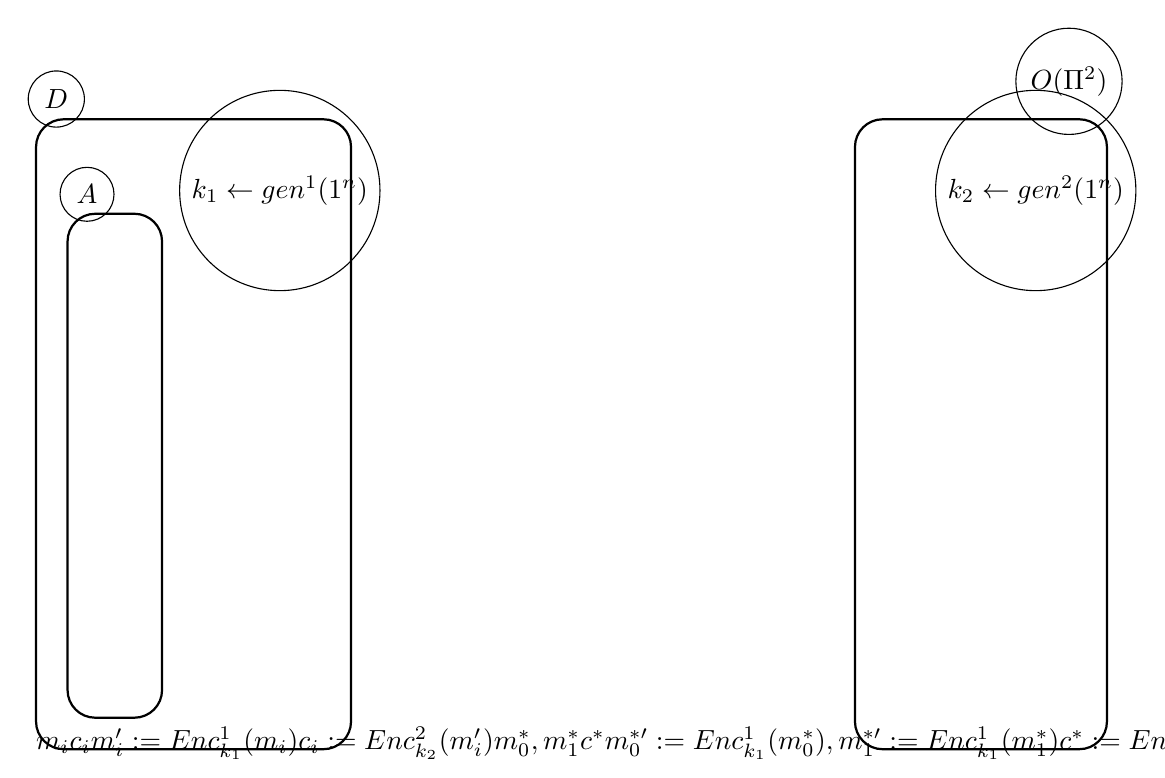
\begin{tikzpicture}[scale=0.8]
			%structure
			\draw[rounded corners=10pt,thick] (0,0) rectangle (5,10);
			\draw[rounded corners=10pt,thick] (0.5,0.5) rectangle (2,8.5);
			\draw[rounded corners=10pt,thick] (13,0) rectangle (17,10);
			\node[above right] at (0,10) {$D$};
			\node[above right] at (0.5,8.5) {$A$};
			\node[above left] at (17,10) {$O(\Pi^2)$};
			\node[below left] at (5,10) {$k_1 \leftarrow gen^1(1^n)$};
			\node[below left] at (17,10) {$k_2 \leftarrow gen^2(1^n)$};
			
			%train phase
			\flect (2,8) -- (4,8) \mess {$m_i$};
			\flect (4,7) -- (2,7) \mess {$c_i$};
			\flect (5,8) -- (13,8) \mess {$m_i':=Enc_{k_1}^1(m_i)$};
			\flect (13,7) -- (5,7) \mess {$c_i:=Enc_{k_2}^2(m_i')$};
			
			%challenge phase
			\flecc (2,5.5) -- (4,5.5) \mess {$m^{\ast}_0,m^{\ast}_1$};
			\flecc (4,4.5) -- (2,4.5) \mess {$c^\ast$};
			\flecc (5,5.5) -- (13,5.5) \mess {$m
			_0^{\ast\prime}:=Enc_{k_1}^{1}(m_0^\ast),m_1^{\ast\prime}:=Enc_{k_1}^{1}(m_1^{\ast})$};
			\flecc (13,4.5) -- (5,4.5) \mess {$c^\ast:=Enc_{k_2}^{2}(m_b^{\ast\prime})$};
			\node[below right] at (13,5.5) {$b \leftarrow \{0,1\}$};
			
			%train phase
			\flect (2,3) -- (4,3) \mess {$m_i$};
			\flect (4,2) -- (2,2) \mess {$c_i$};
			\flect (5,3) -- (13,3) \mess {$m_i':=Enc_{k_1}^1(m_i)$};
			\flect (13,2) -- (5,2) \mess {$c_i:=Enc_{k_2}^2(m_i')$};
			
			% output
			\flec (2,1) -- (3,1) node[pos=1,right] {$b'$};
			\flec (5,1) -- (6,1) node[pos=1,right] {$b''=b'$};
		\end{tikzpicture}
	\end{center}
	As we can see in every case, the distinguisher will have the same probability to find the message encrypted by the oracle than the attacker to break the scheme. As the attacker can only have a probability of $1/2 + \varepsilon$ to succeed the distinguisher will have the same probability. So, the scheme $\Pi$ is secure.
	
	\item As seen in the previous development, if $\Pi^2$ is CPA secure, $\Pi$ is CPA secure. There is no restriction on $\Pi^1$ in that case. Therefore $\Pi^1$ could be such that $Enc^1_{k_1}(m):=m$ which is obviously not CPA secure. So the proposition is false.
	
	\item Idem
	
	\item \textbf{If $\Pi^1$ is CPA secure, is it $\Pi'$ CPA secure?}\\
	The $\Pi'$ scheme is CPA secure if and only if $\Pi^2$ is also CPA secure.
	
	For example, if $Enc_{k_2}^2(m) = m$ then the scheme $\Pi'$ is not CPA secure.
	
	TO DEVELOP. (solution of the teaching assistant?)
	
	\item TODO
	
	\item TODO
	
	\item TODO
\end{enumerate}

\end{solution}


\section{TP 2}
%\addcontentsline{toc}{section}{TP 2}


% \section*{Rappel}

% \begin{center}
% \textbf{Liste des équivalences logiques} 
% \end{center}

% \textsf{Lois commutatives}
% \begin{enumerate}
% 	\item $p \vee q \Lleftarrow\!\!\!\!\Rrightarrow q \vee p$ \textit{(commutativité de $\vee$)}
% 	\item $p \wedge q \Lleftarrow\!\!\!\!\Rrightarrow q \wedge p$ \textit{(commutativité de $\wedge$)}
% 	\item $p \Leftrightarrow q \Lleftarrow\!\!\!\!\Rrightarrow q \Leftrightarrow q$ \textit{(commutativité de $\Leftrightarrow$)}
% \end{enumerate}

% \textsf{Lois associatives}
% \begin{enumerate}
% 	\item $(p \vee q) \vee r \Lleftarrow\!\!\!\!\Rrightarrow p \vee (q \vee r)$ \textit{(associativité de $\vee$)}
% 	\item $(p \wedge q) \wedge r \Lleftarrow\!\!\!\!\Rrightarrow p \wedge (q \wedge r)$ \textit{(associativité de $\wedge$)}
% \end{enumerate}

% \textsf{Lois distributives}
% \begin{enumerate}
% 	\item $p \wedge (q \vee r) \Lleftarrow\!\!\!\!\Rrightarrow (p \wedge q) \vee (p \wedge r)$ \textit{(distributivité de $\wedge$ sur $\vee$)}
% 	\item $p \vee (q \wedge r) \Lleftarrow\!\!\!\!\Rrightarrow (p \vee q) \wedge (p \vee r)$ \textit{(distributivité de $\vee$ sur $\wedge$)}
% \end{enumerate}

% \textsf{Lois de De Morgan}
% \begin{enumerate}
% 	\item $\neg(p \wedge q) \Lleftarrow\!\!\!\!\Rrightarrow \neg p \vee \neg q$ \textit{(loi 1 de De Morgan)}
% 	\item $\neg(p \vee q) \Lleftarrow\!\!\!\!\Rrightarrow \neg p \wedge \neg q$ \textit{(loi 2 de De Morgan)}
% \end{enumerate}

% \textsf{Loi de la négation}
% \begin{enumerate}
% 	\item $\neg \neg p \Lleftarrow\!\!\!\!\Rrightarrow p$
% \end{enumerate}

% \textsf{Loi du tiers exclu}
% \begin{enumerate}
% 	\item $p \vee \neg p \Lleftarrow\!\!\!\!\Rrightarrow \textbf{true} $
% \end{enumerate}

% \textsf{Loi de la contradiction}
% \begin{enumerate}
% 	\item $p \wedge \neg p \Lleftarrow\!\!\!\!\Rrightarrow \textbf{false}$
% \end{enumerate}

% \textsf{Loi de l'implication}
% \begin{enumerate}
% 	\item $p \Rightarrow q \Lleftarrow\!\!\!\!\Rrightarrow \neg p \vee q$
% \end{enumerate}

% \textsf{Loi du contraposée}
% \begin{enumerate}
% 	\item $p \Rightarrow q \Lleftarrow\!\!\!\!\Rrightarrow \neg q \Rightarrow \neg p$
% \end{enumerate}

% \textsf{Loi de l'équivalence}
% \begin{enumerate}
% 	\item $p \Leftrightarrow q \Lleftarrow\!\!\!\!\Rrightarrow (p \Rightarrow q) \wedge (q \Rightarrow p)$
% \end{enumerate}

% \textsf{Lois de l'idempotence}
% \begin{enumerate}
% 	\item $p \Lleftarrow\!\!\!\!\Rrightarrow p \vee p$ \textit{(idempotence de $\vee$)}
% 	\item $p \Lleftarrow\!\!\!\!\Rrightarrow p \wedge p$ \textit{(idempotence de $\wedge$)}
% \end{enumerate}
	
% \textsf{Lois de simplification}
% \begin{enumerate}
% 	\item $p \wedge \textbf{true} \Lleftarrow\!\!\!\!\Rrightarrow p$
% 	\item $p \vee \textbf{true} \Lleftarrow\!\!\!\!\Rrightarrow \textbf{true}$
% 	\item $p \wedge \textbf{false} \Lleftarrow\!\!\!\!\Rrightarrow \textbf{false}$
% 	\item $p \vee \textbf{false} \Lleftarrow\!\!\!\!\Rrightarrow p$
% 	\item $p \vee (p \wedge q) \Lleftarrow\!\!\!\!\Rrightarrow p$
% 	\item $p \wedge (p \vee q) \Lleftarrow\!\!\!\!\Rrightarrow p$
% \end{enumerate}

% \begin{center}
% \textbf{Liste des règles d'inférence}
% \end{center}

% \begin{tabular}{c c c c}

% \textsf{Conjonction} & \textsf{Simplification} & \textsf{Addition} & \textsf{Syllogisme disjoint}   \\

% \begin{tabular}{l}
% $p$ \\
% $q$ \\
% \hline
% $p \wedge q$
% \end{tabular}

% &

% \begin{tabular}{l}
% $p \wedge q$ \\
% \hline
% $p$
% \end{tabular}

% &

% \begin{tabular}{l}
% $p$ \\
% \hline
% $p \vee q$
% \end{tabular}

% &

% \begin{tabular}{l}
% $p \vee q$ \\
% $\neg p$ \\
% \hline
% $q$
% \end{tabular} \\

% \textsf{Modus ponens} & \textsf{Modus tollens} & \textsf{Contradiction} & \textsf{Double négation} \\

% \begin{tabular}{l}
% $p \Rightarrow q$ \\
% $p$ \\
% \hline
% $q$
% \end{tabular}

% &

% \begin{tabular}{l}
% $p \Rightarrow q$ \\
% $\neg q$ \\
% \hline
% $\neg p$
% \end{tabular}

% &

% \begin{tabular}{l}
% $p$ \\
% $\neg p$ \\
% \hline
% $q$
% \end{tabular}

% &
% \begin{tabular}{l}
% $\neg \neg p$ \\
% \hline
% $p$
% \end{tabular} \\

% \textsf{Transitivité} & \textsf{Lois de l'équivalence} & \textsf{Théorème de la déduction} & \textsf{Réduction à l'absurde} \\

% \begin{tabular}{l}
% $p \Leftrightarrow q$ \\
% $q \Leftrightarrow r$ \\
% \hline
% $p \Leftrightarrow r$
% \end{tabular}

% &

% \begin{tabular}{l}
% $p \Leftrightarrow q$ \\
% \hline
% $p \Rightarrow q$ \\
% $q \Rightarrow p$
% \end{tabular}

% &

% \begin{tabular}{l}
% $p, \ldots, r, \boxed{s} \vdash t$ \\
% \hline
% $p, \ldots, r \vdash s \Rightarrow t$
% \end{tabular}

% &

% \begin{tabular}{l}
% $p, \ldots, q, \boxed{r} \vdash s$ \\
% $p, \ldots, q, \boxed{r} \vdash \neg s$ \\
% \hline
% $p, \ldots, q \vdash \neg r$
% \end{tabular}

% \end{tabular}

% \newpage
% \section*{Exercices}

\subsection*{Exercice 1}
Démontrez les équivalences logiques suivantes.

\begin{enumerate}
	\item $p \wedge (q \wedge r)  \Lleftarrow\!\!\!\!\Rrightarrow (p \wedge q) \wedge r$
	\item $p \Rightarrow (q \Rightarrow r) \Lleftarrow\!\!\!\!\Rrightarrow (p \Rightarrow q) \Rightarrow (p \Rightarrow r)$
	\item $p \wedge (p \Rightarrow q) \Rightarrow q \Lleftarrow\!\!\!\!\Rrightarrow \textbf{true}$
	\item $(p \vee q) \wedge (\neg p \vee q) \Lleftarrow\!\!\!\!\Rrightarrow q$
	\item $(p \vee q) \vee (\neg p \wedge \neg q) \Lleftarrow\!\!\!\!\Rrightarrow \textbf{true}$
% 	\item $(p \vee q) \wedge (\neg p \wedge \neg q) \Lleftarrow\!\!\!\!\Rrightarrow \textbf{false}$
	\item $p \vee (q \wedge r) \Lleftarrow\!\!\!\!\Rrightarrow \neg (\neg (p \vee q) \vee \neg (p \vee r))$
	\item $(p \vee q) \wedge \neg (p \wedge q) \Lleftarrow\!\!\!\!\Rrightarrow (p \wedge \neg q) \vee (\neg p \wedge q)$
	\item $p \wedge q \Lleftarrow\!\!\!\!\Rrightarrow (p \vee q) \wedge (p \Leftrightarrow q)$
\end{enumerate}

    \subsubsection*{Solution}
    Notons d'abord que toutes les preuves suivantes peuvent aussi être réalisées grâce aux table de vérités.
\begin{enumerate}
	\item 
    \begin{flalign*}
    p \land (q \land r) &\Lleftarrow\!\!\!\!\Rrightarrow \lnot \lnot (p \land ( q \land r )) \tag*{Double négation}\\
    &\Lleftarrow\!\!\!\!\Rrightarrow \lnot ( \lnot (q \land r) \lor \lnot p ) \tag*{De Morgan}\\
    & \Lleftarrow\!\!\!\!\Rrightarrow \lnot ((\lnot r \lor \lnot q) \lor \lnot p) \tag*{De Morgan} \\
    & \Lleftarrow\!\!\!\!\Rrightarrow \lnot(( \lnot p \lor \lnot q) \lor \lnot r) \tag*{Associativité}\\
    & \Lleftarrow\!\!\!\!\Rrightarrow \lnot (\lnot p \lor \lnot q) \land \lnot \lnot r \tag*{De Morgan} \\
    & \Lleftarrow\!\!\!\!\Rrightarrow (p \land q) \land r \tag*{De Morgan et double négation}
    \end{flalign*}
    
	\item 
	\begin{flalign*}
    p \Rightarrow (q \Rightarrow r)& \Lleftarrow\!\!\!\!\Rrightarrow p \Rightarrow (\lnot q \lor r) \tag*{Implication} \\
    & \Lleftarrow\!\!\!\!\Rrightarrow \lnot p \lor (\lnot q \lor r) \tag*{Implication} \\
    & \Lleftarrow\!\!\!\!\Rrightarrow (\lnot p \lor \lnot q) \lor r \tag*{Associativité}\\
    & \Lleftarrow\!\!\!\!\Rrightarrow (\text{true} \land (\lnot p \lor \lnot q)) \lor r \tag*{Simplification inverse} \\
    & \Lleftarrow\!\!\!\!\Rrightarrow ((\lnot p \lor p) \land  (\lnot p \lor \lnot q)) \lor r \tag*{Loi du tiers exclus}\\
    & \Lleftarrow\!\!\!\!\Rrightarrow (\lnot p \lor (p \land \lnot q)) \lor r \tag*{Distributivité}\\
    & \Lleftarrow\!\!\!\!\Rrightarrow ((p \lor \lnot q) \lor \lnot p) \lor r \tag*{Associativité} \\
    & \Lleftarrow\!\!\!\!\Rrightarrow (p \land \lnot q) \lor (\lnot p \lor r) \tag*{Associativité} \\
    & \Lleftarrow\!\!\!\!\Rrightarrow \lnot \lnot (p \land \lnot q) \lor (\lnot p \lor r) \tag*{Double négation} \\
    & \Lleftarrow\!\!\!\!\Rrightarrow \lnot (\lnot p \lor q ) \lor ( \lnot p \lor \lnot r) \tag*{De Morgan}\\
    & \Lleftarrow\!\!\!\!\Rrightarrow (p \Rightarrow q) \Rightarrow (p \Rightarrow r) \tag*{Implication}
    \end{flalign*}
    
	\item 
	\begin{flalign*}
    p \land (p \Rightarrow q ) \Rightarrow q & \Lleftarrow\!\!\!\!\Rrightarrow p \land (\lnot p \lor q ) \Rightarrow q \tag*{Implication} \\
    & \Lleftarrow\!\!\!\!\Rrightarrow \lnot (p \land ( \lnot p \lor q )) \lor q \tag*{Implication}\\
    & \Lleftarrow\!\!\!\!\Rrightarrow \lnot p \lor \lnot ( \lnot p \lor q ) \lor q \tag*{De Morgan}\\
    & \Lleftarrow\!\!\!\!\Rrightarrow \lnot p \lor (p \land \lnot q) \lor q \tag*{De Morgan}\\
    & \Lleftarrow\!\!\!\!\Rrightarrow (( \lnot p \lor p ) \land ( \lnot p \lor \lnot q )) \lor q \tag*{Distributivité}\\
    & \Lleftarrow\!\!\!\!\Rrightarrow (\text{true} \land ( \lnot p \lor \lnot q )) \lor q \tag*{Loi du tiers exclu}\\
    & \Lleftarrow\!\!\!\!\Rrightarrow ( \lnot p \lor \lnot q ) \lor q \tag*{Simplification}\\
    & \Lleftarrow\!\!\!\!\Rrightarrow \lnot p \lor (\lnot q \lor q ) \tag*{Associativité}\\
    & \Lleftarrow\!\!\!\!\Rrightarrow \lnot p \lor \text{true} \tag*{Loi du tiers exclu}\\
    & \Lleftarrow\!\!\!\!\Rrightarrow \text{true} \tag*{Simplification}\\
    \end{flalign*}
    
	\item 
    \begin{flalign*}
    (p \lor q) \land (\lnot p \lor q) & \Lleftarrow\!\!\!\!\Rrightarrow (q \lor p) \land (q \lor \lnot p) \tag*{Loi commutative}\\
    & \Lleftarrow\!\!\!\!\Rrightarrow q \lor (p \land \lnot p) \tag*{Distributivité}\\
    & \Lleftarrow\!\!\!\!\Rrightarrow q \lor \text{false} \tag*{Simplification}\\
    & \Lleftarrow\!\!\!\!\Rrightarrow q \tag*{Simplification}
    \end{flalign*}
    
	\item 
    \begin{flalign*}
    (p \vee q) \vee (\neg p \wedge \neg q) & \Lleftarrow\!\!\!\!\Rrightarrow (p \vee q) \vee \neg ( p \vee q) \tag*{De Morgan} \\
    & \Lleftarrow\!\!\!\!\Rrightarrow \text{true} \tag*{Loi du tiers exclu}
    \end{flalign*}
    
	\item 
    \begin{flalign*}
    \lnot ( \lnot ( p \lor q ) \lor \lnot (p \lor r ) ) & \Lleftarrow\!\!\!\!\Rrightarrow (p \lor q ) \land ( p \lor r) \tag*{De Morgan}\\
    & \Lleftarrow\!\!\!\!\Rrightarrow p \lor ( q \land r ) \tag*{Distributivité}
    \end{flalign*}
    
	\item 
    \begin{flalign*}
    (p \lor q) \land \lnot ( p \land q) & \Lleftarrow\!\!\!\!\Rrightarrow \lnot (\lnot (p \lor q ) \lor (p \land q)) \tag*{Double négation et De Morgan}\\
    & \Lleftarrow\!\!\!\!\Rrightarrow \lnot (( \lnot p \land \lnot q) \lor ( p \land q)) \tag*{De Morgan}\\
    & \Lleftarrow\!\!\!\!\Rrightarrow \lnot ((\lnot p \lor p) \land (\lnot p \lor q) \land (\lnot q \lor p) \land (\lnot q \lor q)) \tag*{Distributivité}\\
    & \Lleftarrow\!\!\!\!\Rrightarrow \lnot (\text{true} \land (\lnot p \lor q) \land (\lnot q \lor p) \land \text{true}) \tag*{Simplification}\\
    & \Lleftarrow\!\!\!\!\Rrightarrow \lnot ((\lnot p \lor q) \land (\lnot q \lor p)) \tag*{Simplification}\\
    & \Lleftarrow\!\!\!\!\Rrightarrow \lnot (\lnot p \lor q) \lor \lnot(\lnot q \lor p) \tag*{De Morgan}\\
    & \Lleftarrow\!\!\!\!\Rrightarrow (p \land \lnot q) \lor ( q \land \lnot p) \tag*{De Morgan}
    \end{flalign*}
    
	\item 
    \begin{flalign*}
    (p \lor q) \land (p \Leftrightarrow q) & \Lleftarrow\!\!\!\!\Rrightarrow (p \lor q) \land (\lnot p \lor q) \land (p \lor \lnot q) \tag*{Double implication + loi de l'équivalence}\\
    & \Lleftarrow\!\!\!\!\Rrightarrow (p \land \lnot p \land p) \lor (p \land \lnot p \land \lnot q) \lor (p \land q \land p) \lor (p \land q \land \lnot q)\\
    & \lor (q \land \lnot p \land p)\lor (q \land \lnot p \land \lnot q) \lor (q \land q \land p) \lor (q \land q \land \lnot q) \tag*{Distributivité}\\
    & \Lleftarrow\!\!\!\!\Rrightarrow \text{false} \lor \text{false} \lor (p \land q \land p) \lor \text{false} \lor \text{false} \lor \text{false} \lor (q \land q \land p) \lor \text{false} \tag*{Simplification}\\
    & \Lleftarrow\!\!\!\!\Rrightarrow (p \land q) \lor (q \land p) \tag*{Simplification}\\
    & \Lleftarrow\!\!\!\!\Rrightarrow (p \land q) \tag*{Simplification}
    \end{flalign*}

\end{enumerate}


\subsection*{Exercice 2}
Démontrez, à l'aide d'une table de vérité, la validité des arguments suivants:

\begin{enumerate}
	\item \enter
	
	\begin{flushleft}
	\begin{tabular}{l}
		$p \vee q$ \\
		$\neg p$ \\
	\hline
	$q$
	\end{tabular}
\end{flushleft}

	
	\item \enter
	
	\begin{flushleft}
	\begin{tabular}{l}
		$p$ \\
		\hline
	$p \vee q$
	\end{tabular}
	
\end{flushleft}

	\item \enter
	
	\begin{flushleft}
	\begin{tabular}{l}
		$p \Rightarrow q$ \\
		$q \Rightarrow r$ \\
	\hline
	$p \Rightarrow r$
	\end{tabular}
	
\end{flushleft}

\end{enumerate}

    \subsubsection*{Solution}
    
    \begin{enumerate}
    	\item \hspace{1em}

    \begin{center}
	\begin{tabular}{cc|ccc}
		$p$ & $q$ & $\lnot p$ & $p \lor q$ & $(\lnot p) \land (p \lor q)$ \\
		\hline
		T&T&F&T&F\\
		T&F&F&T&F\\
		F&\color{red}T&T&T&\color{red}T\\
		F&F&T&F&F\\
	\end{tabular}
    \end{center}
    
    On remarque que quand $(\lnot p) \land (p \lor q)$ est vrai, $q$ est vrai.
    
	\item  \hspace{1em}
    \begin{center}
    	\begin{tabular}{cc|c}
    		$p$ & $q$ & $p \lor q$ \\
    		\hline
    		\color{red}T&T&\color{red}T\\
    		\color{red}T&F&\color{red}T\\
    		F&T&T\\
    		F&F&F\\
    	\end{tabular}
    \end{center}
    
    On remarque que quand $p$ est vrai, $p \lor q$ est vrai.
    
	\item  \hspace{1em}
    \begin{center}
    	\begin{tabular}{ccc|cccc}
    		$p$ & $q$ & $r$ & $(p \Rightarrow q)$ & $\land$ & $(q \Rightarrow r)$ & $(p \Rightarrow r)$ \\
    		\hline
    		T&T&T&T&\color{red}T&T&\color{red}T\\
    		T&T&F&T&F&F&F\\
    		T&F&T&F&F&T&T\\
    		T&F&F&F&F&T&F\\
    		F&T&T&T&\color{red}T&T&\color{red}T\\
    		F&T&F&T&F&F&T\\
    		F&F&T&T&\color{red}T&T&\color{red}T\\
    		F&F&F&T&\color{red}T&T&\color{red}T\\
    	\end{tabular}
    \end{center}
    
    On remarque que quand $(p \Rightarrow q) \land (q \Rightarrow r)$ est vrai, $(p \Rightarrow r)$ est vrai.
    
    
\end{enumerate}
\subsection*{Exercice 3}
Démontrez que les arguments suivants ne sont pas valides.

\begin{enumerate}
	\item \enter
	
	\begin{flushleft}
	\begin{tabular}{l}
		$p \vee q$ \\
		$\neg p$ \\
	\hline
	$\neg q$
	\end{tabular}
	
\end{flushleft}

	\item \enter
	
	\begin{flushleft}
	\begin{tabular}{l}
		$p \Leftrightarrow q$ \\
		$p \Rightarrow r$ \\
	$r$ \\
	\hline
	$p$
	\end{tabular}
	
\end{flushleft}

	
% 	\item \enter
% 	
% 	\begin{flushleft}
% 	\begin{tabular}{l}
% 		$p \vee q$ \\
% 		$q$ \\
% 	\hline
% 	$p$
% 	\end{tabular}
% 	
% \end{flushleft}

	\item \enter
	
	\begin{flushleft}
	\begin{tabular}{l}
		$p \Rightarrow q$ \\
		$q \Rightarrow p$ \\
	\hline
	$p \wedge q$
	\end{tabular}
	
\end{flushleft}

% 	\item \enter
% 	
% 	\begin{flushleft}
% 	\begin{tabular}{l}
% 		$p \Rightarrow q$ \\
% 		$q$ \\
% 	\hline
% 	$p$
% 	\end{tabular}
% \end{flushleft}

\end{enumerate}

    \subsubsection*{Solution}
    Il y a deux façons de résoudre cet exercice.
    Nous faisons avec le premier un exemple de ces deux méthodes.
\begin{enumerate}
	\item 
    Tout d'abord, l'algorithme de preuve :

    \begin{center}
    \begin{tabular}{|l|l|}
    \hline
    1. $p \lor q$ & Prémisse \\
    2. $\lnot p$ & Prémisse \\
    \hspace{0.5cm} 3. $\lnot q$ & Hypothèse \\
    \hspace{0.5cm} 4. $p$ & Syllogisme disjoint (1, 3) \\ 
    5. $q$ & Réduction à l'absurde \\
    \hline
    \end{tabular}
    \end{center}

    Ensuite une table de vérité :

    \begin{center}
    	\begin{tabular}{cc|ccc|c}
    		$P$ & $Q$ & $(P \lor Q) $ & $\land$ & $\neg P$ & $\neg Q$ \\
    		\hline
    		T & T & T & F & F & F\\
    		T & F & T & F & F & T\\
    		F & T & T & \color{red}T & T & \color{red}F\\ 
    		F & F & F & F & T & T\\
    	\end{tabular}
    \end{center}
    
    On constate que lorsque $(P \lor Q) \land \neg P$ est vrai, $\neg Q$ est faux.
    
	\item 
    Il suffit de trouver une interprétation où c'est faux. Ici on peut prendre :
    
    \begin{flalign*}
    VAL_{I}(p) &= \text{false}\\
    VAL_{I}(q) &= \text{false}\\
    VAL_{I}(r) &= \text{true}\\
    \end{flalign*}
    
    Les prémisses sont vraies, pas la conclusion.
    
	\item 
    Il suffit de trouver une interprétation où c'est faux. Ici on peut prendre :
    
    \begin{flalign*}
    VAL_{I}(p) &= \text{false}\\
    VAL_{I}(q) &= \text{false}\\
    \end{flalign*}
    
    Les prémisses sont vraies, pas la conclusion.
\end{enumerate}

\subsection*{Exercice 4}
Pour chaque ensemble de prémisses, démontrez la conclusion qui suit. Faites attention à bien identifier les
lois logiques et les règles d'inférence utilisées.
\begin{enumerate}

% \item Premisses: $A \vee B \vee C, \ \neg A, \ \neg B$ \\
% 			Conclusion: $C$
% \item Premisses: $(p \wedge q) \vee r$ \\
%       Conclusion: $\neg q \Rightarrow r$
\item Premisses: $p \Rightarrow q$, \ $q \Rightarrow r$ \\
      Conclusion: $p \Rightarrow r$
\item Premisses: $p \Rightarrow q$, \ $r \Rightarrow t$, \ $q \vee t \Rightarrow u$, \ $\neg u$ \\
      Conclusion: $\neg p \wedge \neg r$
\item Premisses: $\neg p \Rightarrow (q \Rightarrow r)$, \ $t \vee \neg r \vee u$, \ $p \Rightarrow t$, \ $\neg t$ \\
      Conclusion: $q \Rightarrow u$
% \item Premisses: $A \Rightarrow B, \ C \Rightarrow D, \ (B \vee D) \Rightarrow E, \ \neg E$ \\
% 			Conclusion: $\neg A \wedge \neg C$
			
			
\item Premisses: $p \Rightarrow \neg q, \ q \vee r \vee s, \ \neg r \vee s \Rightarrow p, \ \neg r$  \\
			Conclusion: $s$
			
			
\item Premisses: $\neg p \Rightarrow (q \Rightarrow r), \ s \vee \neg r \vee t, \ p \Rightarrow s, \ \neg s$ \\
			Conclusion: $q \Rightarrow t$
			
			
%   \item Premisses: $p \wedge q$ \\
%        ronclusion: $p \vee q$
%  \item Premisses: $(p \wedge q) \vee r$ \\
%        ronclusion: $r \vee q$
 \item Premisses: $\neg ( \neg p \wedge q), \ \neg (\neg q \vee r)$ \\
       Conclusion: $p$
%  \item Premisses: $p \vee q$ \\
%        ronclusion: $p \vee \neg \neg q$
 \item Premisses: $p \vee q, \ \neg q \vee r$ \\
       Conclusion: $p \vee r$
 \item Premisses: $(p \wedge q) \vee (r \wedge s), \ (q \wedge r) \vee (s \wedge t)$ \\
       Conclusion: $r \vee (p \wedge t)$

\end{enumerate}

    \subsubsection*{Solution}
    \begin{enumerate}
    
    %%% 4.1 %%%
	\item  \hspace{1em}
    \begin{center}
    \begin{tabular}{|l|l|}
    \hline
    1. $p \Rightarrow q$ & Prémisse \\
    2. $q \Rightarrow r$ & Prémisse \\
    \hspace{0.5cm} 3. $p$ & Hypothèse \\
    \hspace{0.5cm} 4. $q$ & Modus ponens (1, 3) \\
    \hspace{0.5cm} 5. $r$ & Modus ponens (2, 4) \\ 
    6. $p \Rightarrow r$ & Théorème de déduction (3, 5) \\
    \hline
    \end{tabular}
    \end{center}
    
    %%% 4.2 %%%
	\item  \hspace{1em}
    \begin{center}
    \begin{tabular}{|l|l|}
    \hline
    1. $p \Rightarrow q$ & Prémisse \\
    2. $r \Rightarrow t$ & Prémisse \\
    3. $q \lor t \Rightarrow u $ & Prémisse \\
    4. $\lnot u$ & Prémisse \\
    5. $\lnot (q \lor t)$ & Modus tollens (3, 4) \\ 
    6. $\lnot q \land \lnot t$ & De Morgan (5) \\
    7. $\lnot t$ & Simplification (6) \\
    8. $\lnot r$ & Modus tollens (2, 7) \\
    9. $\lnot q$ & Simplification (6) \\
    10. $\lnot p$ & Modus tollens (1, 9) \\
    11. $\lnot r \land \lnot p$ & Conjonction (8, 10) \\
    \hline
    \end{tabular}
    \end{center}
    
    %%% 4.3 %%%
	\item  \hspace{1em}
    \begin{center}
    \begin{tabular}{|l|l|}
    \hline
    1. $\lnot p \Rightarrow (q \Rightarrow r)$ & Prémisse \\

    2. $t \lor \lnot r \lor u$ & Prémisse \\
    3. $p \Rightarrow t$ & Prémisse \\
    4. $\lnot t$ & Prémisse \\
    5. $\lnot p$ & Modus tollens (3, 4) \\ 
    6. $q \Rightarrow r$ & Modus ponens (1, 5) \\
    7. $\lnot r \lor u$ & Syllogisme disjoint (2, 4) \\
    \hspace{0.5cm} 8. $q$ & Hypothèse \\
    \hspace{0.5cm} 9. $r$ & Modus ponens (6, 8) \\
    \hspace{0.5cm} 10. $u$ & Syllogisme disjoint (7,9) \\
    11. $q \Rightarrow u$ & Déduction (8, 10) \\
    \hline
    \end{tabular}
    \end{center}
    
    %%% 4.4 %%%
	\item  \hspace{1em}
    \begin{center}
    \begin{tabular}{|l|l|}
    \hline
    1. $p \Rightarrow \lnot q$ & Prémisse \\
    2. $q \lor r \lor s$ & Prémisse \\
    3. $\lnot r \lor s \Rightarrow p$ & Prémisse \\
    4. $\lnot r$ & Prémisse \\
    5. $q \lor s$ & Syllogisme disjoint (2, 4) \\
    6. $\lnot r \lor s$ & Addition(4) \\
    7. $p$ & Modus ponens (3, 6) \\
    8. $\lnot q$ & Modus ponens (1, 7) \\
    9. $s$ & Syllogisme disjoint (5, 8) \\
    \hline
    \end{tabular}
    \end{center}
    
    %%% 4.5 %%%
	\item  \hspace{1em}
    \begin{center}
    \begin{tabular}{|l|l|}
    \hline
    1. $\lnot p \Rightarrow (q \Rightarrow r)$ & Prémisse \\
    2. $s \lor \lnot r \lor t$ & Prémisse \\
    3. $p \Rightarrow s$ & Prémisse \\
    4. $\lnot s$ & Prémisse \\
    5. $\lnot p$ & Modus tollens (3, 4) \\ 
    6. $q \Rightarrow r$ & Modus ponens (1, 5) \\
    7. $\lnot r \lor t$ & Syllogisme disjoint (2, 4) \\
    \hspace{0.5cm} 8. $q$ & Hypothèse \\
    \hspace{0.5cm} 9. $r$ & Modus ponens (6, 8) \\
    \hspace{0.5cm} 10. $t$ & Syllogisme disjoint (7,9) \\
    11. $q \Rightarrow t$ & Déduction (8, 10) \\
    \hline
    \end{tabular}
    \end{center}
    
    %%% 4.6 %%%
	\item  \hspace{1em}
    \begin{center}
    \begin{tabular}{|l|l|}
    \hline
    1. $\lnot ( \lnot p \land q)$ & Prémisse \\
    2. $\lnot ( \lnot q \lor r)$ & Prémisse \\
    3. $p \lor \lnot q$ & De Morgan (1) \\
    4. $q \land \lnot r$ & De Morgan (2) \\
    5. $q$ & Simplification (4) \\
    6. $p$ & Syllogisme disjoint (3, 5) \\
    \hline
    \end{tabular}
    \end{center}
    
    %%% 4.7 %%%
	\item  \hspace{1em}
    \begin{center}
    \begin{tabular}{|l|l|}
    \hline
    1. $p \lor q$ & Prémisse \\
    2. $\lnot q \lor r$ & Prémisse \\
    3. $q \Rightarrow r$ & Loi de l'implication (2) \\
    \hspace{0.5cm} 4. $\lnot(p \lor r)$ & Hypothèse \\
    \hspace{0.5cm} 5. $\lnot p \land \lnot r$ & De Morgan (4) \\ 
    \hspace{0.5cm} 6. $\lnot p$ & Simplification (5) \\
    \hspace{0.5cm} 7. $\lnot r$ & Simplification (5) \\
    \hspace{0.5cm} 8. $q$ & Syllogisme disjoint (1, 6) \\
    \hspace{0.5cm} 9. $\lnot q$ & Syllogisme disjoint (2, 7) \\
    10. $p \lor r$ & Réduction à l'absurde (4)\\
    \hline
    \end{tabular}
    \end{center}
    
    %%% 4.8 %%%
	\item  \hspace{1em}
    \begin{center}
    \begin{tabular}{|l|l|}
    \hline
    1. $(p \land q) \lor (r \land s)$ & Prémisse \\
    2. $(q \land r) \lor (s \land t)$ & Prémisse \\
    3. $(p \lor r) \land (p \lor s) \land (q \lor s) \land (q \lor r)$ & Distributivité (1) \\
    4. $(q \lor s) \land (q \lor t) \land (r \lor s) \land (r \lor t)$ & Distributivité (2) \\
    5. $p \lor r$ & Simplification (3) \\ 
    6. $r \lor t$ & Simplification (4) \\ 
    7. $(p \lor r) \land (r \lor t)$ & Conjonction (5, 6) \\ 
    8. $r \lor (p \land t)$ & Distributivité (7) \\ 
    \hline
    \end{tabular}
    \end{center}
\end{enumerate}

\subsection*{Exercice 5}
Pour chaque ensemble de prémisses, démontrez la conclusion qui suit. Faites attention à bien identifier les
lois logiques et les règles d'inférence utilisées.
\begin{enumerate}
\item Premisses: \\
      Conclusion: $p \vee \neg (p \wedge q)$
\item Premisses: \\
      Conclusion: $(p \wedge q) \vee \neg p \vee \neg q$
\item Premisses: \\
      Conclusion: $\neg p \vee \neg (\neg q \wedge (\neg p \vee q))$
\end{enumerate}

    \subsubsection*{Solution}
    \begin{enumerate}
    
	\item  \hspace{1em}
    \begin{center}
    \begin{tabular}{|l|l|}
    \hline
    \hspace{0.5cm} 1. $\neg p$ & Hypothèse \\
    \hspace{0.5cm} 2. $\neg p \lor \neg q$ & Addition (1) \\
    \hspace{0.5cm} 3. $\neg \neg(\neg p \lor \neg q)$ & Négation (2) \\
    \hspace{0.5cm} 4. $\neg(p \land q)$ & De Morgan (3)\\ 
    5. $\neg p \Rightarrow \neg(p \land q)$ & Déduction (1, 4) \\
    6. $\neg \neg p \lor \neg(p \land q)$ & Implication (5)\\
    7. $p \lor \neg(p \land q)$ & Double négation (6)\\
    \hline
    \end{tabular}
    \end{center}

	\item  \hspace{1em}
    \begin{center}
    \begin{tabular}{|l|l|}
    \hline
    \hspace{0.5cm} 1. $\neg (p \land q)$ & Hypothèse \\
    \hspace{0.5cm} 2. $\neg p \lor \neg q$ & De Morgan (1) \\
    3. $\neg (p \land q) \Rightarrow (\neg p \lor \neg q)$ & Déduction (1, 2) \\
    4. $(\neg \neg(p \land q)) \lor (\neg p \lor \neg q)$ & Implication (3) \\ 
    5. $(p \land q) \lor (\neg p \lor \neg q)$ & Double négation (4) \\
    \hline
    \end{tabular}
    \end{center}

	\item  \hspace{1em}
    \begin{center}
    \begin{tabular}{|l|l|}
    \hline
    \hspace{0.5cm} 1. $p$ & Hypothèse \\
    \hspace{0.5cm} 2. $p \lor q$ & Addition (1) \\
    \hspace{0.5cm} 3. $(\neg p \lor q) \Leftrightarrow q$ & ex. 2.1 \\
    \hspace{0.5cm} 4. $((\neg p \lor q) \land \neg q) \Leftrightarrow (q \land \neg q)$ & Mystification \\ 
    \hspace{0.5cm} 5. $\neg ((\neg p \lor q) \land \neg q)$ & Contradiction \\
    6. $p \Rightarrow \neg ((\neg p \lor q) \land \neg q)$ & Déduction (1, 5) \\
    7. $\neg p \lor \neg ((\neg p \lor q) \land \neg q)$ & Implication (6) \\
    \hline
    \end{tabular}
    \end{center}
    
    \end{enumerate}


\paragraph*{NB:} Ce qui suit est la correction TP 3 qui a été mise sur Moodle par erreur par l'assistant. Et ce en attente d'une retranscription

\newpage
\addcontentsline{toc}{section}{TP 3}
%Inserer TP3 ICI
\includepdf{TP/TP3_SOL_CUT.pdf} 
\newpage

\section{}
\subsection{Exercise 1 (Authenticated encryption, August 2019 exam)}

\begin{enumerate}
	\item Let $F\colon \K \times \bset^n \mapsto \bset^n$ be a PRF. Consider the following Authenticated Encryption scheme $\Pi=(\Gen, \Enc, \Dec)$ as follow:
	\begin{itemize}
		\item $\Gen$: pick a key uniformly at random in $\K$;
		\item $\Enc$: on input $m$ and $k$:
		\begin{itemize}
			\item Parse $m$ in $l$ blocks $m_1,\dots,m_l$ with $|m_1|=\dots=|m_l|=n$
			\item Pick $r$ uniformly at random in $\bset^{\frac{n}{2}}$
			\item For $i=1,\dots,l$:

				\hspace{1cm} $c_i=F_k(r||i) \oplus m_i$
			\item $c_{l+1}=F_k(r||l+1) \oplus \left(\oplus_{i=1}^l m_i\right)$
			\item Return $(r, c)$ with $c=(c_1,\dots,c_l,c_{l+1})$.
		\end{itemize}
		\item $\Dec$ consequently.
	\end{itemize}
	[For simplicity we suppose that for every message all blocks are \emph{full}, that is, when parsed the last block has length $n$ (i.e., $|m_l|=n$).

	When we write r||i we mean that the number $i$ is written in binary notation putting as many zeros on the left as necessary.]

	\begin{enumerate}
		\item Is $\Pi$ unforgeable? Prove or confute\footnote{*refute}.
		\item Is $\Pi$ CCA-secure? Prove or confute with an attack. [Hint: the previous answer may be useful\dots]
	\end{enumerate}

	\item Let $\Pi'=(\Gen', \Enc', \Dec')$ be an authenticated encryption scheme with binary messages of length $n$. For two binary vectors of length $n$ we denote $\oplus$ the coordinate-wise XOR. $1_n$ denotes the all-$1$ vector of length $n$. Consider the following schemes:
	\begin{itemize}
		\item $\Pi^1 \define (\Gen^1, \Enc^1, \Dec^1)$:
		\begin{itemize}
			\item $\Gen^1 \define \Gen'$,
			\item $\Enc^1_k(m) \define (c_1, c_2) = (\Enc'_k(m), \Enc'_k(m\oplus 1_n))$,
			\item $\Dec^1_k((c_1, c_2)) \define \Dec'_k(c_1)$ if $\Dec'_k(c_1)\oplus \Dec'_k(c_2)=1_n$, $\bot$ otherwise.
		\end{itemize}
		\item $\Pi^2 \define (\Gen^2, \Enc^2, \Dec^2)$:
		\begin{itemize}
			\item $\Gen^2 \define \Gen'$,
			\item $\Enc^2_k(m) \define \Enc'_k(m \oplus 1_n)$,
			\item $\Dec^2_k(c) \define 1_n$ if $\Dec'_k(c)=\bot$, $\Dec'_k(c)\oplus 1_n$ otherwise.
		\end{itemize}
	\end{itemize}
	\begin{enumerate}
		\item Is $\Pi^1$ an authenticated encryption scheme? If not, explain which property you can break and how.
		\item Is $\Pi^2$ an authenticated encryption scheme? If not, explain which property you can break and how.
	\end{enumerate}
\end{enumerate}

% TODO
\begin{solution}
	Note: in the following adversary descriptions, we skip the description of the unused phases of the security games.
	\begin{enumerate}
		\item Notice that there is a constraint on the size of $l+1$: $|l+1| \le \frac{n}{2} \implies l < 2^{n/2}-1$ and thus $|m|=n\cdot l < n\cdot (2^{n/2}-1)$.
		This constraint doesn't play a role in the proofs however.

		\begin{enumerate}
			\item Obviously, for two messages of the same length $m$ and $m'$, we have that \[\forall 1 \le i \le l\colon c'_i = m'_i \oplus F_k(r||i) = (m_i\oplus m'_i) \oplus m_i \oplus F_k(r||i) = (m_i\oplus m'_i) \oplus c_i.\]
			And,
			\begin{align*}
				c'_{l+1} &= F_k(r||l+1) \oplus (\oplus_{i=1}^l m'_i) = F_k(r||l+1) \oplus (\oplus_{i=1}^l m_i) \oplus \left((\oplus_{i=1}^l m_i) \oplus (\oplus_{i=1}^l m'_i)\right) \\
				&= c_{l+1} \oplus \oplus_{i=1}^l (m_i\oplus m'_i).
			\end{align*}
			So, we can build a forgery as follows:
			\begin{enumerate}
				\item Ask to the oracle for the encryption of a message, say, $m=0_n$ ($n$ times the bit $0$) so that it consists of only one block, and receive the answer $(r, c)$.
				\item Output $(r, c^*)$ with $c^* = c \oplus (0_n \oplus 1_n) = c \oplus 1_n = c \oplus m^*$, which is the encryption of message $m^*=1_n$.
			\end{enumerate}
			By construction, it is a forgery with probability 1. So, the scheme is not unforgeable.

			It is also possible to build a forgery by using a message such that $m_{l}=\oplus_{i=1}^{l-1} m_i$;
			then, $c_{l+1}=F_k(r||l+1) \oplus 0^n$, while $c_l=F_k(r||(l-1)+1)\oplus \oplus_{i=1}^{l-1} m_i$,
			and so we can send $(r, c^*)$ with $c^*=(c_1, c_2, \dots, c_{l})$: we drop the last $c_{l+1}$.

			\item In a similar manner, we can build an adversary winning against the CCA game (adversary's viewpoint):
			\begin{enumerate}
				\item The challenger-oracle picks $k \define \Gen(1^n) \pick \bset^n$ uniformly at random.
				\item Output the messages\footnote{We use the notation $m^0$ instead of $m_0$ to differenciate between a message and a message block.}
				$m^0=0_n$ and $m^1=1_n$, and get the challenge ciphertext $(r, c)=\Enc_k(m_b)=(r, c_1, c_2)=(r, F_k(r||1)\oplus m_b, F_k(r||2)\oplus m_b)$.
				\item Ask to the oracle the decryption of $(r, c^*)$ where $c^*=(c_1\oplus 0_{n-1}||1, c_2\oplus 0_{n-1}||1)$. We get its answer as $m^*$. This is of course not the same ciphertext as $c$.
				\item If $m^*=0_{n-1}||1$, output $0$, else ($m^*=1_{n-1}||0$), output $1$.
			\end{enumerate}
			By construction, in building $c^*$ we have constructed the encryption of $m_b\oplus 0_{n-1}||1$, so we flipped the last bit of the encrypted message, allowing us to decrypt it.
			So the probability $\Pr[\PrivKcca(n)=1]=1$, the adversary is PPT, and we have broken CCA security.

			Could we also break CPA security? No (90\% sure), and we can proof it by reduction (distinguisher of $g$ between PRF $F_k$ and random function $f$, based on adversary $A_\Pi$ against $\Pi$).
			Remark that, in the case that the ``PRF'' is a true random function, then each of the $g(r||i)$ are independent random values, and thus the $c_i$ are also independent random value, and so no relation can be found between them in a single message (the ciphertext is just purely random), and the only attack is to hope for a reused $r$.

			Note that the fact that $c_{l+1}$ uses $F_k(r||l+1)$ and not $F_k(r||l)$ is important, because otherwise there would be a reuse of argument, and we can build an attack that even breaks eavesdropper security.
		\end{enumerate}
		\item \begin{enumerate}
			\item $\Pi^1$ is not CCA-secure, and so is not an authenticated encryption scheme; our PPT adversary $\A$:
			\begin{enumerate}
				\item Key generation, as always.
				\item Output $m_0=0_n$ and $m_1=1_n$.

				Receive the challenge $c=(c_1, c_2)=(\Enc'_k(m_b), \Enc'_k(m_b\oplus 1_n))$.
				\item Ask for the decryption of $c'=(c_2, c_1)\neq c$ and receive $m'$. Observe that
				\begin{align*}
					c' &= (\Enc'_k(m_b\oplus 1_n), \Enc'_k(m_b)) = (\Enc'_k(m_b\oplus 1_n), \Enc'_k((m_b\oplus 1_n)\oplus 1_n)) \\
					&= \Enc^1_k(m_b\oplus 1_n) = \Enc^1_k(m_{1-b}).
				\end{align*}
				\item Output $0$ if $m'=m_1$, otherwise $1$ ($m'=m_0$).
			\end{enumerate}
			By construction, $\Pr[\PrivKcca[\A, \Pi^1](n)=1]=1$, which is a non-negligible advantage.

			The scheme is also forgeable, in the same way: simply ask for encryption of $m_0$, receive $c$, then build $c'$ as above: this is a valid ciphertext.

			\item $\Pi^2$ is forgeable, and so it not an authenticated encryption scheme; our PPT adversary $\A$:
			\begin{enumerate}
				\item Key generation, as usual.
				\item Output a random ciphertext $c$.
			\end{enumerate}
			There are two cases:
			\begin{itemize}
				\item either $c$ is the encryption of some message $m$ by $\Enc'_k(\cdot)$, and so $\Dec^2_k(c)=m\oplus 1_n$, and thus it is a valid ciphertext;
				\item or $c$ is not a valid ciphertext for $\Pi'$, in which case $\Dec'_k(c)=\bot$, and thus $\Dec_k(c)=1_n$, which means that $c$ is also a valid ciphertext for $\Pi^2$.
			\end{itemize}
			Thus, in both cases, this random $c$ is a valid ciphertext, and so $\Pr[\EncForge_{\A, \Pi^2}(n)=1]=1$: the scheme is forgeable.

			The fact that, when $\Dec'_k(c)=\bot$, we return $1_n$ instead of a more correct $\bot$, allows us to break the unforgeability.

			Is the scheme CCA-secure?
			Other than this issue, $\Enc^2$ is the same as $\Enc$, and the only exploitable change in behaviour between $\Pi'$ and $\Pi^2$ is the fact that, on $\Pi'$ invalid encryptions, $\Pi^2$ returns $1_n$.
			The only way an adversary could use this particularity would be if he asks for the decryption of an invalid ciphertext (generated at random by him, or by flipping a bit in a valid ciphertext), and he would always get the same $1_n$ answer, not very helpful.
			So the scheme is CCA-secure, and we can further prove it by doing a proof by reduction.
			% TODO do the proof by reduction; 95% sure it works
		\end{enumerate}
	\end{enumerate}
\end{solution}



% OK
% FIXME has been moved from TP5
% Note : this is from TP5 2018-2019, but TP4 2019-2020.
\subsection{Exercise 2 (Authenticated Encryption and sPRP)}

Consider the following scheme $\Pi=(\Gen,\Enc,\Dec)$ based on the strong pseudorandom permutation $\F \colon \K \times \lbrace 0,1 \rbrace^n$, defined as follow:
\begin{itemize}
	\item $\M=\bset^{\frac{n}{2}}$ (the message space)
	\item $\Gen$ picks a random key $k \in \K$
	\item $\Enc_k(m)$ picks a random value $r \in \bset^{\frac{n}{2}}$, and computes $c \define \F_k(m \| r)$
	\item $\Dec_k(c)$ computes $(m\|r)=\F^{-1}_k(c)$ and outputs $m$ (the first half).
\end{itemize}
Answers the following questions:
\begin{itemize}
	\item is $\Pi$ unforgeable?
	\item is $\Pi$ CCA-secure? (\emph{To do at home})
	\item is $\Pi$ an authenticated encryption scheme? (\emph{To do at home})
\end{itemize}

\paragraph{Definition 1} \label{def: sprp} (\emph{Strong PseudoRandom Permutation})

A function $\F \colon \K \times \M \mapsto \M$ is a $(q,t,\negl)$-\emph{ strong pseudorandom permutation} ($\sprp$) if for any $(q,t)$-bounded adversary, the advantage:
\[ \mathsf{Adv}^{\sprp}_{\adv}\define
\left| \Pr\left[ \adv^{\F_k(\cdot),\F_k^{-1}(\cdot)}\Rightarrow 1 \right] -
\Pr\left[ \adv^{\f(\cdot,\cdot),\f^{-1}(\cdot,\cdot)}\Rightarrow 1 \right] \right|
\leq \negl \]
with $k$  and $\f$ picked uniformly at random from their domains, respectively $\K$ and the set of permutations $\M \mapsto \M$.


\begin{solution}
	\begin{enumerate}
		\item It is not unforgeable because since $F_k$ is a PRP, it is bijective (i.e., every image has a pre-image). Then
		\[ \forall c \in \bset, \exists m, r \colon F_k^{-1}(c) = (m || r) \]
		and $\Pr[\EncForge_{\A, \Pi}(n)=1] = 1$.

		\item It is CCA-secure and we will prove it by reduction, assuming that the PRP $F$ is strong.
		Thus, assume we have a PPT adversary $\A$ against the scheme $\Pi$ with advantage $\negl_\A(n)$. Then, we can build a PPT distinguisher $\D$ between a sPRP and a random function, which plays the sPRP game as follows:
		\begin{enumerate}
			\item The challenger-oracle picks $k \define \Gen(1^n) \in \K$, and $b \pick \bset$. If $b=0$, then the challenger uses a true random function $f$ for $g$, if $b=1$, the challenger uses the sPRP $F_k(\cdot)$ for $g$.
			\item First query phase:

			When $\A$ asks for the encryption of a message $m$, $\D$ picks $r \pick \bset^{\frac{n}{2}}$ uniformly at random and queries its oracle on input $m || r$ obtaining, $c = g(m || r)$. $\D$ then forwards $c$ to $\A$.

			When $\A$ asks for the decryption of ciphertext $c$, $\D$ queries its oracle on input $c$ obtaining $m||r=g^{-1}(c)$, and $\D$ answers $m$ to $\A$.

			\item When $\A$ does the challenge query and outputs $m^*_0$, $m^*_1$ with $|m^*_0| = |m^*_1|=\frac{n}{2}$ and $m^*_0 \neq m^*_1$,
			$\D$ picks $r^* \pick \bset^{\frac{n}{2}}$ uniformly at random, and $b' \pick \bset$ uniformly at random too.
			$\D$ queries then its oracle on input $m^*_{b'} || r^*$ obtaining $c^*=g(m^*_{b'}||r^*)$. $\D$ forwards $c^*$ to $\A$.

			\item Second query phase, like the first one, except that $\A$ cannot ask for $\Dec_k(c^*)$.

			\item At the end of the game, $\A$ outputs its guess $b''$. $\D$ outputs $1$ iff $b''=b'$, $0$ otherwise: did the adversary $\A$ guess our correct pick of $b'$?.
		\end{enumerate}
		Let's compute the probability of success for $\D$:
		\begin{itemize}
			\item If $b=0$, then $g=f$, a random function, and so, each ciphertext generated by $g$ and each decrypted message generated by $g^{-1}$ is a random number, independent of each other. In this condition, the best thing the adversary $\A$ can do is wait for a collision on $m||r$ and thus $\Pr[\D \text{ outputs } 1 | b=0]=\Pr[b''=b']=\Pr[\PrivKcca(n)=1]=\frac12 + \frac{q(n)}{2^{n/2}}$.
			\item If $b=1$, then $g=F_k$, and $\A$ is in the right conditions (its interface is respected) to have the advantage $\negl_\A$: $\Pr[\D \text{ outputs } 1 | b=1]=\Pr[b''=b']=\Pr[\PrivKcca(n)=1]=\frac12 + \negl_\A$.
		\end{itemize}
		Thus, the difference between the probabilities is
		\[ \negl_\D(n) = \abs{ \Pr[\D^{F_k(\cdot), F^{-1}_k(\cdot)}(1^n)=1] - \Pr[\D^{f(\cdot), f^{-1}(\cdot)}(1^n)=1] } = \abs{ \negl_\A(n) - \frac{q(n)}{2^{n/2}} } \]
		As we assume that $\F$ is a strong PRP, that the whole construction above is PPT, then $\negl_\D(n)$ must be negligible, and thus the right-hand side must be negligible, and thus $\negl_\A$ must be negligible. The scheme is thus CCA-secure.

		\item Since the scheme $\Pi$ is CCA-Secure but not unforgeable, it is not an authenticated encryption
	\end{enumerate}
\end{solution}



\subsection{Exercise 3 (Hash functions from\ldots hash functions)}

Let $H_2\colon\bset^{2l}\mapsto\bset^{l}$ and $H_3\colon\bset^{3l}\mapsto\bset^{l}$ be
collision resistant hash functions. For $2l$-bit strings $x_i$'s, consider the following two constructions.
\begin{itemize}
	\item $H_4\colon\bset^{4l}\mapsto\bset^{l}$;
	$x=x_1||x_2\rightarrow H_2\left(H_2(x_1)||H_2(x_1\oplus x_2)\right)$
	\smallskip
	\item $H_6\colon\bset^{6l}\mapsto\bset^{l}$;
	$x=x_1||x_2||x_3\rightarrow H_3\left(H_2(x_1\oplus x_2)||H_2(x_2\oplus x_3)||H_2(x_3\oplus x_1)\right)$
\end{itemize}
Determine whether these hash functions are still collision resistant or not.


\begin{solution}
	\begin{itemize}
		\item
		Let's show that from a collision of $H_4$, we generate a collision for $H_2$
		which prove that $H_4$ is collision resistant since $H_2$ is so.
		Let's suppose that we have $x_1\|x_2 \neq y_1\|y_2$ are such that $H_4(x_1\|x_2) = H_4(y_1\|y_2)$.
		\begin{itemize}
			\item
			If $H_2(x_1) \| H_2(x_1 \xor x_2) \neq H_2(y_1) \| H_2(y_1 \xor y_2)$,
			we have a collision for $H_2$ since their image by $H_2$ is identical.
			\item
			If $H_2(x_1) \| H_2(x_1 \xor x_2) = H_2(y_1) \| H_2(y_1 \xor y_2)$,
			we have $H_2(x_1) = H_2(y_1)$ \emph{and} $H_2(x_1 \xor x_2) = H_2(y_1 \xor y_2)$.
			\begin{itemize}
				\item If $x_1 \neq y_1$, we have a collision for $x_2$ since $H_2(x_1) = H_2(y_1)$.
				\item If $x_1 = y_1$, then $x_2 \neq y_2$ since $x_1\|x_2 \neq y_1\|y_2$.
				Therefore $x_1 \xor x_2 \neq y_1 \xor y_2$ and we have collision on $H_2$.
			\end{itemize}
		\end{itemize}
		\item
		$H_6$ is not collision resistant since $H_6(x_1\|x_2\|x_3) = H_6((x_1 \xor w)\|(x_2 \xor w)\|(x_3 \xor w))$
		for all $w$ (collision if $w\neq 0^{2l}$).
		Indeed, since $\xor$ is associative and commutative,
		\begin{align*}
		& = H_6((x_1 \xor w)\|(x_2 \xor w)\|(x_3 \xor w))\\
		& = H_3(H_2((x_1 \xor w) \xor (x_2 \xor w))\|H_2((x_2 \xor w) \xor (x_3 \xor w))\|H_2((x_3 \xor w) \xor (x_1 \xor w)))\\
		& = H_3(H_2(x_1 \xor (w \xor w) \xor x_2)\|H_2(x_2 \xor (w \xor w) \xor x_3)\|H_2(x_3 \xor (w \xor w) \xor x_1)))\\
		& = H_3(H_2(x_1 \xor x_2)\|H_2(x_2 \xor x_3)\|H_2(x_3 \xor x_1)))\\
		& = H_6(x_1\|x_2\|x_3).
		\end{align*}
	\end{itemize}
\end{solution}



\subsection{Exercise 4 (Block-cipher based hash function)}

Considering a block cipher
$E\colon\K\times\M\mapsto\C$; $(k,m)\rightarrow E(k,m)=\Enc_k(m)$
with $\K=\M=\C=\bset^l$, one may try to construct
a collision resistant compression function from $\bset^{2l}$ to $\bset^{l}$.
Show that the following methods do not work :
\[ f_1(x,y)=E(y,x)\oplus y \quad\text{ and }\quad f_2(x,y)=E(x,x)\oplus y \]
That is, show an efficient algorithm for constructing collisions for $f_1$ and $f_2$.
Recall that the block cipher $E$ and the corresponding decryption algorithm $D$ are both
known to you (and they are bijective functions).


\begin{solution}
	We will give 2 collisions for $f_1$ and $f_2$.

	We know that $E(k, \cdot)$ is surjective because it must be injective and $\M = \C$.
	Therefore the decryption exists for all $c \in \C$! We will use it for the second collision of $f_1$.

	For $f_1$, we have the 2 following collisions
	\begin{align*}
	f_1(D(E(y,x),y), E(y,x))
	& = E(E(y,x), D(E(y,x), y)) \xor E(y,x)\\
	& = y \xor E(y,x)\\
	& = E(y,x) \xor y\\
	& = f_1(x, y)\\
	f_1(D(0, E(y,x) \xor y), 0)
	& = E(0, D(0, E(y, x) \xor y)) \xor 0\\
	& = E(y, x) \xor y\\
	& = f_1(x, y).
	\end{align*}
	and for $f_2$ we have
	\begin{align*}
	f_2(x, E(x,x)) & = E(x,x) \xor E(x,x)\\
	& = 0 & \forall x \in \{0,1\}^l\\
	f_2(y, E(x,x)) & = E(y,y) \xor E(x,x)\\
	& = E(x,x) \xor E(y,y)\\
	& = f_2(x, E(y,y)).
	\end{align*}

	\textbf{Other approach:}

	For $f_1$: Let's define $k_1$ and $k_2$ such that $k_2$ is equal to $k_1$ except for the last bit which is flipped. Let's now take an arbitrary $x_1$ for which we ask the encryption $T_{x_1} = E(k_1,x_1)$. Now let's flip the last bit of $T_{x_1}$ and call the result $T_{x_2}$. We can now ask for the decryption of $T_{x_2}$ given $k_2$ as input key, which we know exists since D is bijective and $\C = \bset^{l}$. We then obtain $x_2$. We can now observe that:
	\begin{align*}
	f_1(x_1, k_1) & = E(k_1,x_1) \xor k_1\\
	& = T_{x_1}  \xor k_1\\
	f_1(x_2, k_2) & = E(k_2,x_2) \xor k_2\\
	& = T_{x_2} \xor k_2\\
	& = (T_{x_1} \xor 0^{l-1}||1 )\:\xor\: (k_1 \xor 0^{l-1}||1)\\
	& = T_{x_1}  \xor k_1
	\end{align*}
	For $f_2$: We can ask for $T_x = \:E(x,x)$ and $T_y = E(y,y)$ for two arbitrary (but different) $x$ and $y$.  We can see that:
	\begin{align*}
	f_2(y, T_x) & = E(y,y) \xor T_x\\
	& = T_y  \xor T_x\\
	f_2(x, T_y) & = E(x,x) \xor T_y\\
	& = T_x \xor T_y
	\end{align*}
	Which are both equal with different input, this is a collision.
\end{solution}



% OK
\subsection{Exercise 5 (Authenticated encryption, or not)}

\copypaste{10}{1}



\subsection{Exercise 6 (Variable-length MAC)}

Considering a known hash function $h^s\colon\bset^{2l}\mapsto\bset^{l}$,
let's note by $H^s$ the corresponding Merkle-Damg{\aa}rd transform hash function,
\emph{i.e.}

\begin{center}
	\begin{tikzpicture}[scale=0.5]
	\tikzstyle{every node}=[text centered, inner sep = 2pt]

	\trapeze{$h^s$}{\position}
	\draw [->] \position +(-3,0) node [left] {$IV$} -- +(-1,0);
	\draw [<-] \position + (-1,1) -| ++(-2,3) node [above] {\mylabel};
	\draw \position + (1,0) -- +(2,0) node {};
	\renewcommand{\position}{(4,0)}
	\renewcommand{\mylabel}{$x_2$}
	\trapeze{$h^s$}{\position}
	\draw [->] \position +(-2,0) node [below] {} -- +(-1,0);
	\draw [<-] \position + (-1,1) -| ++(-2,3) node [above] {\mylabel};
	\draw [->]\position + (1,0) -- +(2,0) node [right] {$\ldots$};
	\renewcommand{\position}{(9.5,0)}
	\renewcommand{\mylabel}{$x_n$}
	\trapeze{$h^s$}{\position}
	\draw [->] \position +(-2.2,0) node [below] {} -- +(-1,0);
	\draw [<-] \position + (-1,1) -| ++(-2,3) node [above] {\mylabel};
	\draw \position + (1,0) -- +(2,0) node {};
	\renewcommand{\position}{(13.5,0)}
	\renewcommand{\mylabel}{$\left|x\right|$}
	\trapeze{$h^s$}{\position}
	\draw [->] \position +(-2,0) node [below] {} -- +(-1,0);
	\draw [<-] \position + (-1,1) -| ++(-2,2.95) node [above] {\mylabel};
	\draw [->] \position + (1,0) -- +(2,0) node [right] {$H^s(x)$};
	\end{tikzpicture}
\end{center}
%
when $x=x_1||\cdots||x_n$ for some integer $n$ and when the $x_i$'s are
$l$-bit strings.

Show why, with a private key $k$ of length $l$, the MAC scheme
\[t \define H^s(k||m),\]
is \emph{not} existentially unforgeable under an adaptive chosen-message attack.


\begin{solution}
	If we have the tag of $p$, which is (let's consider that $k$ and $p$ are $l$ bits long for simplicity)
	\[ t_p = H^s(k\|p) = h^s(h^s(h^s(IV \| k) \| p) \| 2l) \]
	we can find the tag of $p\|2l\|w$ (where $w$ is $l$ bits long for simplicity)
	without knowing $k$ since we know $h^s$ (it is public knowledge, only the secret $k$ is secret and requires an oracle).
	It is
	\begin{align*}
		H^s(k\|p\|2l\|w)
		& = h^s(h^s(h^s(h^s(h^s(IV \| k) \| p) \| 2l) \| w) \| 4l)\\
		& = h^s(h^s(H^s(k \| p) \| w) \| 4l)\\
		& = h^s(h^s(t_p \| w) \| 4l)
	\end{align*}
	Since $p\|2l\|w \neq p$, this gives us an existential forgery.
\end{solution}



% OK
\subsection{Exercise 7 (Hash-MAC)}

Suppose $H_0$ and $H_1$ are compression functions but only one is believed to be collision resistant.
Besides, suppose $\textsc{Mac}_0$ and $\textsc{Mac}_1$ are message authentication codes but only one
of the both schemes is known to be unforgeable. Is it possible to build a secure ''hash-MAC'' from these
inputs? Justify your answer.

%Homework 2 of Dan Boneh, Winter 2011, Problem 5 (DVD security)
\begin{solution}
	We build $H(m) = H_0(m)\|H_1(m)$.
	If we have $m_1 \neq m_2$ such that $H(m_1) = H(m_2)$ then $H_0(m_1) = H_0(m_2)$ and
	$H_1(m_1) = H_1(m_2)$ so the collision resistant hash function has a collision whichever it is.
	However, $H$ is no more a compression function and we cannot use Merkle-Damg\aa{}rd.

	The fact that we don't know the compressive factor also prevents us from building (simply) Merkle-Damg\aa{}rd or sponge constructions based on each of the functions.

	The input of $H$ therefore cannot have arbitrary length but its output is twice the length of the output of $H_0$ and $H_1$ so it is twice the size of a tag.

	The output of $\Mac_0$ and $\Mac_1$ are the size of a tag so we can use the tag
	$H(\Mac_0(k,m)\|\Mac_1(k,m))$ for our Hash-MAC scheme.
	If we are able to output an existential forgery $(m, t)$, since $H$ is collision resistant, that means that we have found $\Mac_0(k,m)\|\Mac_1(k,m)$ and therefore we have found an existential forgery for both $\Mac_0$ \emph{and} $\Mac_1$ which is absurd since one of them is believed to be unforgeable.

	Our Hash-MAC scheme is therefore unforgeable.
\end{solution}



\subsection{Exercise 8 (Blue-ray security)}

\copypaste{3}{7}

\section{}

The TP5 of 2019-2020 reviewed the basics of number theory and group theory for this course. As they are not really useful for the exam and are fairly trivial (once the basics are know, that is), they are skipped in this document.

Below are the exercises of last year pertaining to groups and number theory.



\subsection{Exercise 0 (Group order)}

\copypaste{3}{5}



\subsection{Exercise 3 (Euclidean algorithm for gcd)}

Let $a,b \in \mathbb{Z}$ , $b \neq 0$, consider the following algorithm, presented in Algorithm~\ref{algo:gcd}. ($r=a \% b$ means that $a=qb+r$ where $q$ is the quotient and $r$ is the remainder).

Prove that $x$, the value returned by Algorithm~\ref{algo:gcd}, is $\mathsf{gcd} (a,b)$.

Hint:
\begin{itemize}
	\item Prove that $x$ divides  $ \mathsf{gcd} (a,b)$
	\item Prove that $ \mathsf{gcd} (a,b)$ divides $x$
\end{itemize}

\begin{algorithm}
	\KwIn{$a$, $b$}
	\KwOut{$\mathsf{gcd}(a,b)$}

	\While{ $b\neq 0$}
	{
		$r \leftarrow a\%b$\;

		$a \leftarrow b$\;

		$b \leftarrow r$\;
	}
	\Return($a$)

	\caption{The Euclidean $\mathsf{gcd}$ algorithm.}\label{algo:gcd}
\end{algorithm}


\begin{solution}
	According to the algorithm, we will have as successive value for the different remainder:
	\[(r_2 = r_0 \% r_1, r_3 = r_1 \% r_2, \ r_4 = r_2 \% r_3, \ ... \ , r_n =  r_{n-2} \% r_{n-1})\]
	Where $r_0 = a$, $r_1 = b$ and $r_n$ is the last non null remainder. Then we have the property that :
	\[ gcd(r_{i}, r_{i+1}) = gcd(r_{i+1}, r_{i+2}) \ \forall i : \ 0 \leq i \leq n - 2 \]
	Otherwise if it was not the case, $\exists i < n $ such that $r_i = 0$. But as $r_n$ is the last non null remainder, we prove by contradiction this property.

	As $gcd(r_{n-1}, r_n) = r_n $ because $r_n | r_{n-1}$ (since $r_{n+1} = r_{n-1} \% r_n = 0$), we can conclude that
	\[ gcd(r_0, r_1) = gcd(a, b) = gcd(r_{n-2}, r_{n-1}) = r_n\]
	We have proved the value returned by the algorithm is the $gcd(a,b)$
\end{solution}



\subsection{Exercise 4}

Consider the group $\mathbb{Z}^{\ast}_{17}$.
\begin{enumerate}
	\item Compute $5^{-1}$.
	\item Compute $3^2$, $3^3$ and $3^4$.
	\item Does $3$ generate the group?
	\item Find $\log_{7}(11)$.
\end{enumerate}


\begin{solution}
	Here because p is not too big, it is possible to evaluate "quickly" and "intuitively" the solutions. If it is too hard, there is an algorithm in the slides.
	\begin{enumerate}
		\item Because 35 mod 17 = 1, and $5 \cdot 7 = 35$. \newline Then $5^{-1} = 7$.  ($5 \cdot 7 = 1 \text{ (mod 17)}$)
		\item \begin{itemize}
			\item $3^2 = 9 \text{ (mod 17)}$
			\item $3^3 = 3^2 \cdot 3 = 27 \text{ (mod 17)} = 10 \text{ (mod 17)}$
			\item $3^3 = 3^3 \cdot 3 = 30 \text{ (mod 17)} = 13 \text{ (mod 17)}$
		\end{itemize}
		\item According to \textit{Fermat's little theorem}, if ord(g) = i then if $i|m = |G|$, where G is the commutative group. To see if 3 generate the group, we have to check if $3^i \neq 1$ where $i$ are the divisor of $(p-1) = 16$ (except 16 of course !).
		\begin{itemize}
			\item $3^1$ = 3 mod 17 (trivial)
			\item $3^2$ = 9 mod 17 (evaluated previously)
			\item $3^4$ = 13 mod 17 (evaluated previously)
			\item $3^8$ = $(3^4)^2$ = $(13)^2 \text{ (mod 17)}$ = $(-4)^2 \text{ (mod 17)}$ = 16 mod 17
		\end{itemize}
		We can see that 3 is a generator of the group.

		\textbf{P.S.} : The trick here is to remember the property of the modulo operation here in a $Z^*_p$:
		\[ x = -(p - x) \text{ (mod p)} \]
		It can make a lot of computing easier (it can become a real pain in the ass).
		\item Here we have to find x such that:
		\[ 7^x = 11 \text{ (mod 17)} \]
		After (boring) computations, we have here :
		\begin{itemize}
			\item $7^1$ = 7 mod 17
			\item $7^2$ = 15 mod 17 = -2 mod 17
			\item $7^3$ = -14 mod 17 = 3 mod 17
			\item $7^4$ = 4 mod 17
			\item $7^5$ = 11 mod 17 (Bingo)
		\end{itemize}
		Then $log_7(11)$ = 5
	\end{enumerate}
\end{solution}



\subsection{Exercise 5 (Group order)}

In this exercise we consider the group $\Z_{59}^*$.

\begin{enumerate}
	\item What is the order of $58$?
	\item What are the possible orders of an element of this group?
	\item Find an element of order more than $20$.
\end{enumerate}


\begin{solution}
	The order of $g \in \Z^*_{59}$ is the smallest $i$ where $g^i = 1$
	\begin{enumerate}
		\item ord(58) = 2 because:
		\begin{itemize}
			\item  $58^1$ = 58 mod 59 = -1 mod 59
			\item  $58^2$ = -58 mod 59 = 1 mod 59
		\end{itemize}
		\item According to \textit{Fermat's little theorem}, the possible orders of a group $\mathbb{Z}^*_{p}$ are the divisor of p-1. Then, the possible orders are:
		\begin{itemize}
			\item 1
			\item 2
			\item 29
			\item 58
		\end{itemize}
		\item The best strategy here is to find a number g where
		\[ ord(g) > 2 \]
		(To assure you this is correct, just look at the possible ordrers).  \newline
		2 is a correct candidate.
	\end{enumerate}
\end{solution}

\section{}
%\addcontentsline{toc}{chapter}{TP 6}

\subsection*{Exercice 1}
Pour chacune des affirmations suivantes, démontrez-la ou trouvez un contre-exemple.
\begin{enumerate}
	\item $\neg \exists x \ \forall y \ p(x, y) \Lleftarrow\!\!\!\!\Rrightarrow \forall x, y \ \neg p(x, y)$
	\item $\exists x \ p(x) \vee q(x) \Rrightarrow (\exists x \ p(x)) \vee (\exists x \ q(x))$
	\item $(\exists x \ p(x)) \wedge (\exists x \ q(x)) \Rrightarrow \exists x \ p(x) \wedge q(x)$
	\item $\forall x \ \exists y \ p(x, y) \Lleftarrow\!\!\!\!\Rrightarrow \exists x \forall y \ p(x, y)$
	\item $(\exists x \ p(x)) \vee (\exists x \ q(x)) \Rrightarrow \exists x \ p(x) \vee q(x)$
\end{enumerate}

    \subsubsection*{Solution}
  
    \paragraph{1)}  
        \begin{tabular}{|l|l|}
        \hline
        $\forall$ x $\neg$ $\forall$ y p(x,y) $\Lleftarrow \Rrightarrow$ $\forall$ x,y $\neg$ p(x,y) & $\neg$ vers l'intérieur\\
        $\forall$ x $\exists$ y $\neg$ p(x,y) $\ne$ $\forall$ x,y $\neg$ p(x,y)& $\neg$ vers l'intérieur\\
        \hline
        \end{tabular}
    
    \paragraph{2)}
        \begin{tabular}{|l|l|}
        \hline
        1. $\exists$x p(x) $\lor$ q(x) & hypothèse \\
        $\qquad$ 2. $\neg$ [$\exists$x p(x) $\lor$ $\exists$x q(x)] & hypothèse absurde\\
        $\qquad$ 3. $\neg$ $\exists$x p(x) $\land$ $\neg$ $\exists$x q(x) & Morgan\\
        $\qquad$ 4. $\forall$x $\neg$ p(x) $\land$ $\forall$x $\neg$ q(x) & $\neg$ vers l'intérieur\\
        $\qquad$ 5. $\forall$x $\neg$ p(x) & simplification\\
        $\qquad$ 6. $\neg$ p(x) & élimination $\forall$\\
        $\qquad$ 7. p(x) $\lor$ q(x) & élimination $\exists$ (1)\\
        $\qquad$ 8. q(x) & Syllogisme disjoint (6,7)\\
        $\qquad$ 9. $\forall$x $\neg$ q(x) & simplification (4)\\
        $\qquad$ 10. $\neg$ q(x) & \\
        11. $\neg \neg$ ( $\exists$x p(x) $\lor$ $\exists$x q(x)) & Preuve par contradiction\\
        12. $\exists$x p(x) $\lor$ $\exists$x q(x)& Simplification\\
        13. $\exists$x p(x) $\lor$ q(x) $\Rrightarrow$ ($\exists$x p(x) $\lor$ ($\exists$x q(x)) & Preuve\\
        \hline
        \end{tabular}
        
    \paragraph{3)}
        Faux, par exemple soit p(x) = x est petit;
        soit q(x) = x est grand. Il existe un $x$ petit, et il existe un $x$ grand, mais pas de $x$ petit et grand à la fois. Il s'agit ici de comprendre que dans le premier cas, la variable $x$ n'est pas la même à cause de la portée de deux quantificateurs, alors que dans le second, c'est bien le même $x$.
        
    \paragraph{4)}
        Faux, par exemple:
        Soit P(x,y) = y est le père de x.
        Si pour tout $x$, il existe un $y$ tel que $y$ est le père de $x$, ce n'est pas pour autant qu'un $x$ aura pour père tous les $y$ possibles.
        
    \paragraph{5)}
        \begin{tabular}{|l|l|}
        \hline
        1. $(\exists xp(x)) \lor (\exists xq(x))$ & Prémisse \\
        \indent 2. $\neg \exists xp(x) \lor q(x)$ & Hypothèse absurde\\
        \indent 3. $\forall x\neg (p(x) \lor q(x))$ & Loi de la négation(2)\\
        \indent 4. $\forall x(\neg p() \land \neg q(x))$ & De Morgan(3) \\
        \indent 5. $\neg p(a) \land \neg q(a)$ & Élimination $\forall$(4) \\
        \indent 6. $\neg p(a)$ & Simplification(5) \\
        \indent 7. $\forall x(\neg p(x)) $ & Introduction $\forall$(6) \\
        \indent 8. $\neg \exists x p(x)$ & Loi de la négation(7) \\
        \indent 9. $\exists x q(x)$ & Syllogisme Disjoint(1, 6)\\
        \indent 10. $q(a)$ & Élimination $\exists$(9)\\
        \indent 11. $\neg q(a)$ & Simplification(5)\\
        12. $\neg \neg \exists xp(x) \lor q(x)$ & Réduction à l'absurde \\
        13. $\exists xp(x) \lor q(x)$ & Simplification(11)\\
        \hline
        \end{tabular}
        
\subsection*{Exercice 2}
Mettez les formules suivantes en forme normale prenexe puis en forme normale de Skolem et finalement en forme clausale. 
\begin{enumerate}
\item $(p(x) \vee \exists x \ q(x)) \Rightarrow \forall z \ r(z)$
\item $(\forall x \ (p(x) \Rightarrow q(x))) \wedge (\exists z \ p(z)) \wedge (\exists z \ (q(z) \Rightarrow r(t)))$
\item $\forall x \ ( ((\exists y \ r(x, y)) \wedge (\forall y \  \neg s(x, y)) \Rightarrow \neg (\exists y \ r(x, y) \wedge P)) )$
\item $\neg \forall x \ \exists y \ f(u, x, y) \Rightarrow (\exists x \ \neg \forall y \ g(y, v) \Rightarrow h(x))$
\end{enumerate}

    \subsubsection*{Solution}
    
    \paragraph{1)}
    \begin{center}
    \begin{tabular}{|l|l|c|}
    \hline
    $(p(x) \lor \exists x \ q(x)) \Rightarrow \forall z \ r(z)$ & Départ & Expression de base \\
    $\neg (p(x) \lor \exists x \ q(x)) \lor (\forall z \ r(z))$ & Suppression de $\Rightarrow$ & \\
    $\neg (p(y) \lor \exists x \ q(x)) \lor (\forall z \ r(z))$ & Renommage des variables & \\
    $(\neg p(y) \land \neg \exists x \ q(x)) \lor (\forall z \ r(z))$ & De Morgan 2 & \\
    $(\neg p(y) \land \forall x \ \neg q(x)) \lor (\forall z \ r(z))$ & $\neg \exists x$ devient  $\forall x \neg$ & \\
    $\forall x \ \forall z \ [(\neg p(y) \land \neg q(x)) \lor r(z)]$ & Extraction des quantificateurs & Forme prénexe\\
    $\forall x \ \forall z \ [(\neg p(y) \land \neg q(x)) \lor r(z)]$ & Pas de changements & Forme de Skolem\\
    $\forall x \ \forall z \ [(\neg p(y) \lor r(z)) \land (\neg q(x) \lor r(z))]$ & Distribution & Forme clausale\\
    \hline
    \end{tabular}
    \end{center}
    
    \paragraph{2)}
    
    \begin{center}
    \begin{tabular}{|l|l|c|}
    \hline
    $(\forall x \ (p(x) \Rightarrow q(x))) \land (\exists z \ p(z)) \land (\exists z \ (q(z) \Rightarrow r(t)))$ & Départ & Expression de base \\
    $(\forall x \ (\neg p(x) \lor q(x))) \land (\exists z \ p(z)) \land (\exists z \ (\neg q(z) \lor r(t)))$ & Suppression $\Rightarrow$ & \\
    $(\forall x \ (\neg p(x) \lor q(x))) \land (\exists y \ p(y)) \land (\exists z \ (\neg q(z) \lor r(t)))$ & Renommage & \\
    $\forall x \ \exists y \ \exists z \ [(\neg p(x) \lor q(x)) \land p(y) \land (\neg q(z) \lor r(t))]$ & Extraction & Forme prénexe \\
    $\forall x \ [(\neg p(x) \lor q(x)) \land p(f(x)) \land (\neg q(g(x)) \lor r(t))]$ & Élimination $\exists$ & Forme de Skolem \\
    $\forall x \ [(\neg p(x) \lor q(x)) \land p(f(x)) \land (\neg q(g(x)) \lor r(t))]$ & Pas de changements & Forme clausale \\
    \hline
    \end{tabular}
    \end{center}
    
    \paragraph{3)}
    \begin{center}
    \begin{tabular}{|l|l|c|}
    \hline
    $\forall x \ [ (\exists y \ r(x, y)) \land (\forall y \  \neg s(x, y)) \Rightarrow \neg (\exists y \ r(x, y) \land P) ]$ & Départ & Expression de base \\
    $\forall x \ [ \neg ((\exists y \ r(x, y)) \land (\forall y \  \neg s(x, y))) \lor \neg (\exists y \ r(x, y) \land P) ]$ & Suppression $\Rightarrow$ & \\
    $\forall x \ [ \neg ((\exists y \ r(x, y)) \land (\forall u \  \neg s(x, u))) \lor \neg (\exists v \ r(x, v) \land P) ]$ & Renommage & \\
    $\forall x \ [ \neg(\exists y \ r(x, y)) \lor \neg (\forall u \  \neg s(x, u)) \lor ( \neg \exists v \ r(x, v) \lor \neg P) ]$ & De Morgan 1 & \\
    $\forall x \ [ (\forall y \ \neg r(x, y)) \lor (\exists u \  s(x, u)) \lor ( \forall v \ \neg r(x, v) \lor \neg P) ]$ & Simplification $\neg$ & \\
    $\forall x \ \forall y \ \exists u \   \forall v \ [ \neg r(x, y) \lor s(x, u) \lor (\neg r(x, v) \lor \neg P) ]$ & Extraction & Forme prénexe \\
    $\forall x \ \forall y \ \exists u \   \forall v \ [ \neg r(x, y) \lor s(x, u) \lor \neg r(x, v) \lor \neg P ]$ & Associativité $\lor$ & \\
    $\forall x \ \forall y \ \exists u \ [ \neg r(x, y) \lor s(x, u) \lor \neg P ]$ & Simplification & \\
    $\forall x \ \forall y \ [ \neg r(x, y) \lor s(x, f(x, y)) \lor \neg P ]$ & Élimination $\exists$ & Forme de Skolem \\
    $\forall x \ \forall y \ [ \neg r(x, y) \lor s(x, f(x, y)) \lor \neg P ]$ & Pas de changements & Forme clausale \\
    \hline
    \end{tabular}
    \end{center}
    
    \paragraph{4)}
    \begin{center}
    \begin{tabular}{|l|l|c|}
    \hline
    $\neg \forall x \ \exists y \ f(u, x, y) \Rightarrow (\exists x \ \neg \forall y \ g(y, v) \Rightarrow h(x))$ & Départ & Expression de base \\
    $\neg \forall x \ \exists y \ [\neg f(u, x, y) \lor (\exists x \ \neg \forall y \ (\neg g(y, v) \lor h(x)))]$ & Suppression $\Rightarrow$ & \\
    $\neg \forall x \ \exists y \ [\neg f(u, x, y) \lor (\exists w \ \neg \forall z \ (\neg g(z, v) \lor h(w)))]$ & Renommage & \\
    $\exists x \ \forall y \ \neg [\neg f(u, x, y) \lor (\exists w \ \exists z \ \neg (\neg g(z, v) \lor h(w)))]$ & Simplification & \\
    $\exists x \ \forall y \ [\neg \neg f(u, x, y) \land \neg (\exists w \ \exists z \ \neg (\neg g(z, v) \lor h(w)))]$ & De Morgan 2 & \\
    $\exists x \ \forall y \ [f(u, x, y) \land (\forall w \ \forall z \ (\neg g(z, v) \lor h(w)))]$ & Simplification & \\
    $\exists x \ \forall y \ \forall w \ \forall z \ [f(u, x, y) \land (\neg g(z, v) \lor h(w))]$ & Extraction & Forme prénexe \\
    $\forall y \ \forall w \ \forall z \ [f(u, x, y) \land (\neg g(z, v) \lor h(w))]$ & Élimination $\exists$ & Forme de Skolem \\
    $\forall y \ \forall w \ \forall z \ [f(u, x, y) \land (\neg g(z, v) \lor h(w))]$ & Pas de changements & Forme clausale \\
    \hline
    \end{tabular}
    \end{center}
    

\subsection*{Exercice 3}
Montrez avec l'algorithme de r\'{e}solution que $p_1 \wedge p_2 \wedge p_3$ est une contradiction o\`{u}
\begin{align*}
p_1 & \equiv \forall x \ p(x, f(x)) \Rightarrow q(x) \\
p_2 & \equiv \forall x \ \forall y \ p(f((x), f(y)) \\
p_3 & \equiv \exists x \ \neg q(f(x))
\end{align*}

    \subsubsection*{Solution}
    
    \textbf{\textit{ 1. Mise en Forme Clausale (FC)}} \\
    . $p_1 \equiv \forall x \ \neg p(x, f(x)) \lor q(x) $\\
    . $p_2 \equiv \forall x \ \forall y \ p(f((x), f(y)) $\\
    . $p_3 \equiv \neg q(f(a_x))$ \\
    
    \textbf{\textit{2. Itérations }} \\
    $ S = Input = \{ \neg p(x, f(x)) \lor q(x), p(f((x), f(y)), \neg q(f(a_x) \} $ \\
    $ \sigma_1 = \{ (x, f(a_x)) \} $ \\
    $ Res( \ ( \neg p(x, f(x)) \lor q(x))\sigma_1, \neg q(f(a_x) \ ) = Res( \ ( \neg p[f(a_x), f(f(a_x))] \lor q[f(a_x)] ), \neg q(f(a_x)  \ ) \\ = \neg p(f(a_x), f(f(a_x))) $  [ajouter cette formule dans S] \\
    $ S = Input = \{ \neg p(x, f(x)) \lor q(x), p[f(x), f(y)], \neg q(f(a_x), \neg p[f(a_x), f(f(a_x))] \} $
     
    \noindent $ \sigma_{2} = \{ (x,a_x), (y,f(a_x) ) \}$\\
    $ Res( \ (p[f(x), f(y)])\sigma_2, \neg p[f(a_x), f(f(a_x))] \ ) \\ = Res( \ p[f(a_x), f(f(a_x))], \neg p[f(a_x), f(f(a_x))] \ ) = FALSE $\\ 
    


\subsection*{Exercice 4}
Montrez avec l'algorithme de r\'{e}solution que si $\forall x \ q(x) \Leftrightarrow p(x)$ et $\exists x \ \neg q(x)$ alors $\exists x \ \neg p(x)$.

    \subsubsection*{Solution}
    
   \textbf{\textit{ 1. Mise en Forme Clausale (FC)}} \\
    . $\forall x \ q(x) \Leftrightarrow p(x)$ et $\exists x \ \neg q(x) \equiv \forall x \ (p(x) \Rightarrow q(x)) \land (q(x) \Rightarrow p(x)) 
     \equiv \forall x \ (\neg p(x) \lor q(x)) \land (\neg q(x) \lor p(x)) $ \\
    . $\exists x \ \neg q(x) \equiv \neg q(a_{x}) $  \\
    . $\neg \exists x \ \neg p(x) \equiv \forall x \ \neg \neg p(x) \equiv \forall x \ p(x) $ [négation de la formule à prouver] \\
    
    \textbf{\textit{2. Itérations }} \\
    $ S = \{ \neg p(x) \lor q(x) , \neg q(x) \lor p(x) ,  \neg q(a_{x}) , p(x) \}  $ \\
    $ \sigma = \{(x, a_{x}) \} $ \\
    $ Res( (\neg p(x) \lor q(x))\sigma , \neg q(a_{x}) ) = \neg p(a_{x}) $ [ajouter cette formule dans S] \\
    $ S = \{ \neg p(x) \lor q(x) , \neg q(x) \lor p(x) ,  \neg q(a_{x}) , p(x), \neg p(a_{x}) \}$  \\
    $ Res( (p(x))\sigma, \neg p(a_{x}) ) = FALSE $ \\


\subsection*{Exercice 5}
Montrez avec l'algorithme de r\'{e}solution que si $\forall x \ p(x) \Rightarrow q(x, y)$, $\forall x \ p(x) \vee r(x)$ et $\neg r(a)$ alors $\exists x \ q(a, x)$.

    \subsubsection*{Solution}
    
     \textbf{\textit{ 1. Mise en Forme Clausale (FC)}} \\
     . $\forall x \ p(x) \Rightarrow q(x, y) \equiv \forall x \ \neg p(x) \lor q(x,y) \equiv \forall x \ \neg p(x) \lor q(x,b)  $ \\
     . $\forall x \ p(x) \lor r(x) $ \\
     . $\neg r(a) $ \\
     . $\neg \exists x \ q(a, x) \equiv \forall x \ \neg q(a,x) $ [négation de la formule à prouver] \\
    
    
    \textbf{\textit{2. Itérations }} \\
    $ S = \{ \neg p(x) \lor q(x,b), p(x) \lor r(x), \neg r(a), \neg q(a,x) \} $\\
    $ \sigma_{1} = \{ (x,a) \}$\\
    $ Res( (p(x) \lor r(x))\sigma_{1}, \neg r(a) ) = p(a) $\\
    $ S = \{ \neg p(x) \lor q(x,b), p(x) \lor r(x), \neg r(a), \neg q(a,x), p(a) \} $\\
    $ Res( (\neg p(x) \lor q(x,b))\sigma_{1}, p(a) )= q(a,b) $\\
    $ S = \{ \neg p(x) \lor q(x,b), p(x) \lor r(x), \neg r(a), \neg q(a,x), p(a), q(a,b) \} $
    
    \noindent $ \sigma_{2} = \{ (x,b) \}$\\
    $ Res( (\neg q(a,x))\sigma_{2}, q(a,b) )= FALSE $\\
    



\section{}


\subsection{Exercise 1 (Commitment scheme)}
\label{subsec:commit-scheme}

Define the bit-commitment scheme $\langle \G, \Com, \Open \rangle$ with the following PPT algorithms:
\begin{itemize}
	\item $\Gen(1^n)$ sets $pk$ as $(\PRG,R)$, where
	\begin{itemize}
		\item $\mathsf{G}$ is a random generator $\lbrace 0,1 \rbrace^n \longmapsto \lbrace 0,1\rbrace^{3n}$
		\item $R$ is a random $3n$-bit string
	\end{itemize}
	\item $\Com_{pk}(b)$ with $b\in\{0,1\}$ provides $(c,d)$ where:
	\begin{itemize}
		\item $Y$ is an $n$-bit string
		\item  if $b=0$ $c=\mathsf{G}(Y)$
		\item if $b=1$, $c=\mathsf{G}(Y) \oplus R$
		\item $d=(b,Y)$
	\end{itemize}
	\item $\Open_{pk}(c,d)$ outputs $b$ if it can recompute $c$ from $d$ and $pk$, or $\bot$ otherwise
\end{itemize}

\begin{enumerate}
	\item Is this scheme perfectly hiding?
	\item Is this scheme computationaly binding?
	\item If the committer choose $R$ is the scheme secure?
\end{enumerate}


\begin{solution}
	\begin{enumerate}
		\item For a scheme to be perfectly hiding, we need that $\forall \A$:
		\[ \Pr[\ComHide_{\A,\Pi}=1]=\frac12 \Leftrightarrow \Pr[c|b=0] = \Pr[c|b=1] \]
		If $b=0$, then $c$ has as much randomness as $\mathsf{G}$, which has as much randomness as $Y$, so $n$ bits of randomnes (=there are $2^n$ possible values for $c$).

		If $b=1$, then $c$ has as much randomness as $\mathsf{G}$ and $R$, so basically $3n$ bits of randomness (=there are $2^{3n}$ possible values for $c$).

		If we have unbounded computational power, then we could enumerate all possible outputs $\mathsf{G}(Y)$, and see if $c$ is in this set of values.
		If $b=0$, we are sure they are in;
		if $c=1$, there are $2^{2n}$ possible $R$ such that $\mathsf{G}(y) \oplus R$ cannot be distinguished from $\mathsf{G}(Y')$ (simply, $R=\mathsf{G}(Y)\oplus \mathsf{G}(Y')$), so there is a probability $\frac{2^{2n}}{2^{3n}}=\frac{1}{2^{n}}$ that $c \in \{\mathsf{G}(Y)\}$.
		So the probability of success for an unbounded adversary is
		\[ \frac{1}{2} \cdot 1 + \frac{1}{2} (1-\frac{1}{2^{n}}) = 1-\frac{1}{2^{n+1}} \]
		So, an unbounded adversary has near-certainty of breaking the hiding property.

		To break the hiding property, an adversary would need to enumerate all possible outputs of $\mathsf{G}$ (requires $2^n$ steps) if $G(Y) \oplus R \notin \{x | \forall u : x = G(u)\}$.

		But this kind of event has a negligible chance of probability ($\Pr = \frac{|\mathsf{G}(Y)|}{|\mathsf{G}(Y) \oplus R|} = \frac{2^n}{2^{3n}} = \frac{1}{2^{2n}} = \negl(n)$) so an adversary with an unbounded power of calculation can easily break the property of perfectly hiding.

		It is however simple to prove that the scheme is computationally hiding.

		\item For the scheme to be computationally binding, it should be intractable to find $(c, d_0, d_1)$ such that $\Open_{pk}(c, d_0)=0$ and $\Open_{pk}(c, d_1)=1$.
		If we replace, we find that it is equivalent to find $Y_0, Y_1$ such that
		\[ c=\mathsf{G}(Y_0) = \mathsf{G}(Y_1) \oplus R \]
		For this to be possible at all, we need to have $R=\mathsf{G}(Y_0) \oplus \mathsf{G}(Y_1)$ for some $Y_0, Y_1$.
		But, we have that $|\{R\}|=2^{3n}$ while $|\{ \mathsf{G}(Y_0) \oplus \mathsf{G}(Y_1) \}| \le 2^{2n}$, so the probability of $R$ being correct for this to happen is at most $\frac{2^{2n}}{2^{3n}}=\frac{1}{2^n}$, which is negligible.
		And so, \[ \Pr[\ComBind_{\A, \Pi}(n)=1] \le \frac{1}{2^n} \quad \forall \A. \]
		So even if we have an adversary capable of finding $Y_0$ and $Y_1$ with near-certainty, the fact that $R$ can just be badly chosen for him causes its probability of success to be \emph{in all cases} negligible.
		So, the scheme is computationally binding.

		\item Not secure, because if the committer chooses $R = G(Y)$, then the opposite player can easily deduce the value of b. If $c = 0$, $b = 1$, else $b = 0$.
	\end{enumerate}
\end{solution}



\subsection{Exercise 2 (Commitment with DL)}

Let $(\mathbb{G}, \cdot)$ be a group in which the discrete logarithm is difficult, with $|\mathbb{G}|=q$.
Let $g$ be a generator of the group and $h$ be a random element of the group ($(g, h)$ may be seen as the key of the hash function).
Define the following hash funtion $\mathsf{H}\colon \Z^*_q \times \Z^*_q \mapsto \mathsf{G}$:
\[ \mathsf{H}_{g,h} (\alpha, \beta) \define g^\alpha h^\beta \]
Prove that if the DL is difficult, then, the hash function is collision resistant.
For simplicity we assume that $q$ is prime.


\begin{solution}
	I don't know, maybe a reduction might be useful? It's been such a long time!

	For the reduction, let's assume that we have an adversary $\A$ that can break the collision resistance by finding a collision with advantage $\negl(2n)$.
	We have $2n$ instead of $n$ because the seed of the hash function has $2n$ bits instead of $n$.
	Then, we can build an adversary $\D$ that can solve the DL problem:
	\begin{enumerate}
		\item Run $\mathcal{G}(1^n)$ to obtain $(\mathbb{G}, q, g)$ where $g$ generates $\mathbb{G}$ of order $q$ with $|q|=n$.
		\item Choose $h \pick \mathbb{G}$.
		\item Send $(\mathbb{G}, q, g, h)$ to $\D$.
		\item $\D$ uses $\A$: he sends $(g, h)$ as the seed.
		Then, with probability $\negl(2n)$, $\A$ answers with $(\alpha, \beta)$ and $(\alpha', \beta')$ such that $\alpha\neq\alpha' \vee \beta\neq\beta'$ and
		\[ g^\alpha h^\beta = g^{\alpha'} g^{\beta'} \]
		From this, if we want to find $x$ such that $g^x=h$, then we just replace:
		\begin{align*}
		g^\alpha (g^x)^\beta &= g^{\alpha'} (g^x)^{\beta'} \\
		\alpha + x \beta &= \alpha' + x \beta' \\
		x &= \frac{\alpha'-\alpha}{\beta-\beta'}
		\end{align*}
	\end{enumerate}
	We have
	\[ \Pr[\DLog_{\D, \mathcal{G}}(n)=1] = \Pr[g^x=h] = \Pr[\HashColl_{\A, \mathsf{H}}(n)=1] = \negl(2n) \le \negl'(n)\]
	And, as we know that the DL problem is hard is $\mathbb{G}$, then we know that these probabilities should be negligible, and so that finding a collision is also hard.
\end{solution}



% OK
\subsection{Exercise 3 (Commitment scheme and batching)}

\copypaste{9}{0}



\subsection{Exercise 4 (Decisional Diffie-Hellman and \texorpdfstring{$\mathbb{Z}_p^\ast$}{Zp*})}

The goals of this exercise are to define $QR_p$, prove some of its properties, and to show that in some groups DDH and CDH assumptions are conjectured not equivalent, as DDH is easy whereas CDH is conjectured to be hard.

\begin{enumerate}
	\item For all element $a$ of $\mathbb{Z}_{11}^*$, compute $a^2 \mod 11$.

	For a prime number $p$, we denote $QR_p$ the set $\{x \in \mathbb{Z}_{p}^* \; | \; \exists a\in \mathbb{Z}_{p}^*, a^2=x\}$, such $x$ are called quadratic residues modulo $p$. Show that if $p$ is odd then $|QR_p|=\frac{p-1}{2}$.

	\item Show that, if $p$ is odd, $QR_p$ is a cyclic group (therefore, $QR_p$ is a subgroup of $\Z^*_p$).

	\item For all element $a$ of $\mathbb{Z}_{11}^*$, compute $a^5 \mod 11$. Show that for any odd prime $p$, $x \in QR_p \Leftrightarrow x^{\frac{p-1}{2}}= 1 \mod p$, and that $x \not \in QR_p \Leftrightarrow x^{\frac{p-1}{2}}= -1 \mod p$.

	\item Show that $2$ is a generator of $\mathbb{Z}_{11}^*$. For the following pairs $(a,b)$, compute $g^a, g^b$ and $g^{ab}$ in $\mathbb{Z}_{11}^*$ where $g=2$:
	\begin{itemize}
		\item $(2,8)$,
		\item $(1,4)$,
		\item $(3,5)$.
	\end{itemize}
	Show that for $p$ an odd prime, $g^{ab} \not \in QR_p \Leftrightarrow g^a \not \in QR_p \text{ and } g^b \not \in QR_p$.

	\item Show that DDH does not hold in $\mathbb{Z}_{p}^*$ with $p$ an odd prime.
\end{enumerate}


% TODO rewrite this to use the official proof
\begin{solution}
	An official solution was given in the exercise session.

	For this exercise we will work with $\Z_{11}^* = \{1,2,3,4,5,6,7,8,9,10\}$
	\begin{enumerate}
		\item
		For all element $a$ of $\Z_{11}^*$, I've calculated $a^2$ mod $11$.
		\[1^2 = 1 \quad 2^2 = 4 \quad 3^2 = 9 \quad 4^2 = 5 \quad 5^2 = 3 \quad 6^2 = 3 \quad 7^2 = 5 \quad 8^2 = 9 \quad 9^2 = 4 \quad 10^2 = 1\]
		We see that with $p$ odd, we have $\left|QR_p\right| = \frac{p-1}{2}$. We can show it with this development:

		\item
		\nosubsolution

		\item
		For all element $a$ of $\Z_{11}^*$, I've calculated $a^5$ mod $11$.
		\[1^5 = 3^5 = 4^5 = 5^5 = 9^5 = 1 \qquad 2^5 = 6^5 = 7^5 = 8^5 = 10^5 = 10\]
		We can see that for $p$ prime, we have $x \in QR_p \Leftrightarrow x^{\frac{p-1}{2}} = 1 \mod p$ and  $x \notin QR_p \Leftrightarrow x^{\frac{p-1}{2}} = p-1 \mod p$.
		\begin{itemize}
			\item $x \in QR_p \Leftrightarrow x^{\frac{p-1}{2}} = 1 \mod p$:\\
			We know that \[x \in QR_p \Leftrightarrow \exists a \st x = a^2 \mod p\]
			So we have now \[x = a^2 \mod p \Leftrightarrow x^{\frac{p-1}{2}} = 1 \mod p\]
			If we replace $x$ by $a$ we obtain $a^{2^{(\frac{p-1}{2})}} = 1 \mod p$.\\
			But also more simply $a^{p-1} = 1 \mod p$ which is true by the group theory.
			\item $x \notin QR_p \Leftrightarrow x^{\frac{p-1}{2}} = p-1 \mod p$:\\
			We know that \[x \notin QR_p \Leftrightarrow \exists a \st x = a^{1+2n} \mod p\]
			So we have now \[x = a^{1+2n} \mod p \Leftrightarrow x^{\frac{p-1}{2}} = -1 \mod p\]
			We replace $x$ by $a$ and we get \[a^{\frac{p-1}{2}} a^{n(p-1)} \mod p = -1 \mod p\]
			We know that $ a^{n(p-1)} \mod p = 1$, thus we simplify the equation like \[a^{\frac{p-1}{2}} \mod p = -1 \mod p\]
			We know that $g = a^{\frac{p-1}{2}} \mod p \ne 1 \mod p$ but $g^2 = a^{p-1} = 1 \mod p$. The only solution of these two equations is $g = -1 \mod p$ which is equivalent to
			\[x^{\frac{p-1}{2}} = p-1 \mod p\]
		\end{itemize}

		\item
		The number $2$ is a generator of $\Z_{11}^*$, because ord($2$) $= 10$. In fact, we have $2^1 = 2$, $2^2 = 4$, $2^5 = 10$ and $2^10 = 1$. (Fermat's little theorem)
		We have $g = 2$ so:
		\begin{itemize}
			\item $(2,8):\quad g^2 = 4$, $g^8 = 3$ and $g^{16} = -2$
			\item $(1,4):\quad g^1 = 2$, $g^4 = 5$ and $g^{4} = 5$
			\item $(3,5):\quad g^3 = -3$, $g^5 = -1$ and $g^{15} = -1$ TODO
		\end{itemize}
		We have to show that $g^{ab} \notin QR_p \Leftrightarrow g^a \notin QR_p \text{ and } g^b \notin QR_p$.\\
		We know by the definition of the $QR_p$ set that
		\[g^n \notin QR_p \Leftrightarrow \exists m \st n = 2m+1\]
		We can thus extract from $g^{ab} \notin QR_p$ that $\exists m \st ab = 2m+1$.

		% not necessary
		%We can do a proof by contradiction:\newline
		%If $a = 2v$ then $ab = 2bv$ and can not be equal to $2m + 1$.\\
		%If $b = 2v$ then $ab = 2av$ and can not be equal to $2m + 1$.\\

		So we are assured that $a$ and $b$ are not pairs, so we have the relation $g^a \notin QR_p \text{ and } g^b \notin QR_p$ if and only if $ab = 2m+1$ which is equivalent to $g^{ab} \notin QR_p$. That was what we had to proof.

		\item
		We have to show that DDH does not hold in $\Z_p^*$ with p an odd prime number.

		We define an attacker that can see $p$, $g$, $g^a$, $g^b$ and receive $h_b = g^{ab}$ or $g^z$.
		The behaviour of the attacker will be this one:
		\begin{itemize}
			\item It receives $g^a \notin QR_p$ and $g^b \notin QR_p$:\\
			It will answer in function of $h_b$:
			\begin{itemize}
				\item $h_b \notin QR_p$:\\
				It answers $h_b = g^{ab}$
				\item $h_b \in QR_p$:\\
				It answers $h_b = g^z$
			\end{itemize}
			\item It receives $g^a \in QR_p$ or $g^b \in QR_p$:\\
			It answers randomly.
		\end{itemize}
		We can identify four cases with their chances of success and appearance (we already know that $\left|QR_p\right|$ is of size $\frac{p-1}{2}$):
		\begin{enumerate}[a)]
			\item $g^a \in QR_p$ or $g^b \in QR_p$ appears $3/4$ of the time with success = $1/2$.
			\item $g^a \notin QR_p$ and $g^b \notin QR_p$ with $h_b = g^{ab}$  appears $1/8$ of the time with success = $1$.
			\item $g^a \notin QR_p$ and $g^b \notin QR_p$ with $h_b = g^z$ and $g^z \in QR_p$  appears $1/16$ of the time with success = $1$.
			\item $g^a \notin QR_p$ and $g^b \notin QR_p$ with $h_b = g^z$ and $g^z \notin QR_p$  appears $1/16$ of the time with success = $0$.
		\end{enumerate}
		We can now recalculate the expected value of success of our attacker:
		\begin{align*}
		\mathbb{E}(success) &= \frac{3}{4}\cdot \frac{1}{2} +  \frac{1}{8}\cdot 1 + \frac{1}{16}\cdot 1 + \frac{1}{16}\cdot 0\\
		&= \frac{1}{2} + \frac{1}{16}
		\end{align*}
		This attacker has one sixteenth of probability more than one half which is not a negligible function (in fact it is a constant function). It is not DDH secure.
	\end{enumerate}
\end{solution}


\subsection{Exercise 5}

\copypaste{8}{1}

% BUG LSTSET
\section{TP 8}
%\addcontentsline{toc}{chapter}{TP 8}



% \subsection*{Exercice }
% Soit l'interpr\'{e}tation suivante: \\
% \begin{center}
% \begin{tabular}{r l}
% $D_I$ & $= \mathbb{N}$ \\
% $val_I(a)$ & $= 0$ \\
% $val_I(f)$ & $= $ \ ''succ`` \\
% $val_I(P)$ & $= $ \ ''$<$`` \\
% $val_I(x)$ & $= 1$ \\
% $val_I(y)$ & $= 0$ \\
% \end{tabular}
% \end{center}
% D\'{e}terminez les valeurs de v\'{e}rit\'{e} des formules suivantes dans cette interpr\'{e}tation:
% \begin{enumerate}
% \item $P(x, a)$
% \item $P(x, a) \wedge P(x, f(x))$
% \item $\exists y \ P(y, x)$
% \item $\exists y \ P(y, a) \vee P(f(y), y))$
% \item $\forall x \ \exists y \ P(x, y)$
% \item $\exists y \ \forall x \ P(x, y)$
% \end{enumerate}
% 
% 
% \vspace{0.5cm}

\subsection*{Exercice 1}
Modelisez les propositions suivantes en prolog.
\footnotesize
\begin{enumerate}
\item $\forall \ X, Y, Z \ american(X) \ \wedge \ weapon(Y) \ \wedge \ sells(X, Y, Z) \ \wedge \ hostile(Z) \Rightarrow criminal(X)$
\item $owns(nono, m1)$
\item $missile(m1)$
\item $\forall X \ missile(X) \ \wedge \ owns(nono, X) \Rightarrow sells(west, X, nono)$
\item $\forall X \ missile(X) \ \Rightarrow weapon(X)$
\item $\forall X \ enemy(X, america) \Rightarrow hostile(X)$
\item $american(west)$
\item $enemy(nono, america)$
\end{enumerate}
\normalsize
Quelles sont les \'{e}tapes que prolog fait pour r\'{e}pondre \`{a} la requ\^{e}te \texttt{criminal(west)}?

    \subsubsection*{Solution}
    
    %\lstset{language=Prolog, frame = single, numbers=left, numbersep=-0.5cm, numberstyle=\small\color{mygray}, escapeinside={\%*}{*)}}
    
    \begin{lstlisting}
    criminal(X) :- american(X), weapon(Y), sells(X, Y, Z), hostile(Z).
    owns(nono, m1).
    missile(m1).
    sells(west, X, nono) :- missile(X), owns(nono, X).
    weapon(X) :- missile(X).
    hostile(X) :- enemy(X, america).
    american(west).
    enemy(nono, america).
    \end{lstlisting}
    
    \subsubsection*{Étapes d'exécution}
    \begin{tabular}{l|l}
    \textit{Requête initiale}& \\
    r0 = <criminal(west)>& \\
    \textit{Résolution 1}& \\
    s1 = {(X,west)} & \textit{X} de \textit{criminal} vaut \textit{west}\\
    r1 = <american(west),weapon(Y),sells(west,Y,Z),hostile(Z)> & Développement de \textit{criminal} \\
    \textit{Résolution 2} &\\
    s2 = s1 & Pas de changement\\
    r2 = <weapon(Y),sells(west,Y,Z),hostile(Z)>  & \textit{american(west)} vaut \textit{true}\\
    \textit{Résolution 3} &\\
    s3 = s2 & Pas de changement\\
    r3 = <missile(Y),sells(west,Y,Z),hostile(Z)> & Développement de \textit{weapon}\\
    \textit{Résolution 4} &\\
    s4 = s3 U {(Y,m1)} & \textit{Y} de \textit{missile} vaut \textit{m1}\\
    r4 = <sells(west,m1,Z),hostile(Z)> & \textit{missile(m1)} vaut \textit{true}\\
    \textit{Résolution 5} &\\
    s5 = s4 U {(Z, nono)} & \textit{Z} de \textit{sells} vaut \textit{nono}\\
    r5 = <missile(m1),owns(nono,m1),hostile(nono)> & Développement de \textit{sells}\\
    \textit{Résolution 6} &\\
    s6 = s5 & Pas de changement\\
    r6 = <owns(nono,m1),hostile(nono)> & \textit{missile(m1)} vaut \textit{true}\\
    \textit{Résolution 7} &\\
    s7 = s6 & Pas de changement\\
    r7 = <hostile(nono)> & \textit{owns(nono,m1)} vaut \textit{true}\\
    \textit{Résolution 8} &\\
    s8 = s7 & Pas de changement\\
    r8 = <enemy(nono,america)> & Développement de \textit{hostile}\\
    \textit{Résolution 9} &\\
    s9 = s8 & Pas de changement\\
    r9 = < > & \textit{ennemy(nono, america)} vaut \textit{true}\\
    \end{tabular}
    
    \noindent La résolvante finale est vide, la requête renvoie \textit{true}
    
    
\subsection*{Exercice 2}
Dans cet exercice on va voir comment d\'{e}finir des pr\'{e}dicats pour l'arithmétique en prolog. On
d\'{e}finit 0 par le symbole \texttt{0}, 1 par \texttt{s(0)}, 2 par \texttt{s(s(0))} etc. On d\'{e}finit
$-x$ par \texttt{negative(x)}. Par example, $-2$ est represent\'{e} par \texttt{negative(s(s(0)))}.

\begin{enumerate}
 \item \'{E}crivez un programme qui fait la somme de deux nombres.
 \item \'{E}crivez un programme qui fait la soustraction de deux nombres.
 \item Comment vous faites pour calculer $a - b$ si $a < b$?.
\end{enumerate}

    \subsubsection*{Solution}
    
    Pour réaliser un programme en Prolog, l'idéal est de réfléchir d'abord au cas de base, puis au cas récursif.
    
    \begin{lstlisting}
    /* Addition */
    add(0, X, X).                            % 0+X=X         
    add(s(X), Y, Z) :- add(X, s(Y), Z).      % (X+1)+Y=Z  <==  X+(Y+1)=Z
    
    /* Soustraction */
    minus(X, 0, X).                          %  X-0=X
    minus(s(X), s(Y), Z) :- minus(X, Y, Z).  % (X+1)-(Y+1)=Z  <==  X-Y=Z
    minus(0, X, negative(X)).                % Cas a < b
    \end{lstlisting}


\subsection*{Exercice 3}
Dans cette exercice on va voir comment d\'{e}finir des pr\'{e}dicats pour des op\'{e}rations sur des listes en
prolog. \'{E}crivez un programme qui:
\begin{enumerate}
 \item ajoute un \'{e}l\'{e}ment dans une liste.
 \item retire le premier \'{e}l\'{e}ment d'une liste.
 \item v\'{e}rifie si une liste contient un \'{e}l\'{e}ment donn\'{e}.
 \item fait la somme des \'{e}l\'{e}ments d'une liste.
 \item fait la concat\'{e}nation de deux listes.
 \item calcule la taille d'une liste.
 \item v\'{e}rifie si deux listes sont les m\^{e}mes.
 \item obtient le $i$-\`{e}me \'{e}l\'{e}ment d'une liste.
\end{enumerate}

    \subsubsection*{Solution}
    
    \begin{lstlisting}
    /* Ajout/Suppression */
    add(X, L, [X|L]).
    remove([X|L], L).
    
    /* Contient */
    contains(X, [X|L]).
    contains(X, [Y|L]) :- contains(X,L).
    
    /* Somme */
    sum([], 0).
    sum([X|L], R) :- sum(L, R1), R is X + R1.
     
    /* Concatenation */
    concat([], L, L).
    concat([X|L1], L2, [X|L3]) :- concat(L1, L2, L3).
    
    /* Taille */
    size([], 0).
    size([X|L], R) :- size(L, R1), R is 1 + R1.
    
    /* Comparaison */
    equal([],[]).
    equal([X|L1],[X|L2]) :- equal(L1, L2).
    
    /* Recuperation element */
    get([X|L], 1, X).
    get([X|L], I, R) :- H is I - 1, get(L, H, R).
    \end{lstlisting}


\subsection*{Exercice 4}
Quel est le r\'{e}sultat de la requ\^{e}te \texttt{concat(X, Y, [1, 2, 3])} pour votre op\'{e}ration \texttt{concat} de l'exercice 3?

    \subsubsection*{Solution}
    \noindent On obtient les résultats suivants :
    \begin{description}
    \item \texttt{X = [\ ],}
    \item \texttt{Y = [1, 2, 3]} 
    \end{description}
    \begin{description}
    \item \texttt{X = [1],}
    \item \texttt{Y = [2, 3]} 
    \end{description}
    \begin{description}
    \item \texttt{X = [1,2],}
    \item \texttt{Y = [3]} 
    \end{description}
    \begin{description}
    \item \texttt{X = [1, 2, 3],}
    \item \texttt{Y = [\ ]} 
    \end{description}


\subsection*{Exercice 5}
On peut mod\'{e}liser un graphe en prolog avec des pr\'{e}dicats \texttt{link(a, b)} pour les ar\^{e}tes du graphe. Par example,
le graphe
\begin{center}
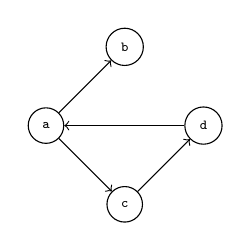
\begin{tikzpicture}
\node[draw, circle] (b) at (0, 0) {\tiny \texttt{b}};
\node[draw, circle] (a) at (-1, -1) {\tiny \texttt{a}};
\node[draw, circle] (d) at (1, -1) {\tiny \texttt{d}};
\node[draw, circle] (c) at (0, -2) {\tiny \texttt{c}};
\draw[->] (a) -- (b);
\draw[->] (a) -- (c);
\draw[->] (c) -- (d);
\draw[->] (d) -- (a);
\end{tikzpicture}
\end{center}
est repr\'{e}sent\'{e} par: \\

\noindent \texttt{link(a, b)}. \\
\texttt{link(a, c)}. \\
\texttt{link(c, d)}. \\
\texttt{link(d, a)}.

\begin{enumerate}
 \item \'{E}crivez un pr\'{e}dicat \texttt{path(X, Y)} qui est vrai s'il exsite un chemin de X \`{a} Y.
 \item Est-ce que l'ordre des pr\'{e}dicats dans votre programme a de l'importance?
 \item Comment calculer le chemin, et pas juste savoir s'il y en a un? Vous pouvez calculer le
 chemin dans l'ordre inverse si c'est plus simple.
 \item Comment on fait pour calculer tous les chemins entre X et Y?
\end{enumerate}

    \subsubsection*{Solution}
    \begin{lstlisting}
    
    /* Partie 1 : Existence */
    
    link(a, b).
    link(a, c).
    link(c, d).
    link(d, a).
    
    path(X, Y) :- link(X, Y).
    path(X, Y) :- link(X, Z), path(Z, Y).
    
    /* Partie 2 : Ordre *
    
    path(X,Y) :- path(Z, Y), link(X, Z).
    %*\text{\% Fonctionne aussi, mais moins efficace.}*)
    %*\text{\% L’ordre des predicats n’a de l’importance que pour les performances.} *)
    
    /* Partie 3 : Chemin */
    
    link(a, b, [a, b]).
    link(a, c, [a, c]).
    link(c, d, [c, d]).
    
    path(X, Z, P) :- link(X, Z, P).
    path(X, Z, [X|P2]) :- link(X, Y, P1), path(Y, Z, P2).
    \end{lstlisting}
    
    \paragraph{4)} Pour calculer tous les chemins, il suffit de lancer le programme de la partie 3, puis d'attendre une réponse.
    Lorsqu'on a une solution, on peut demander au programme de revenir en arrière et de modifier son dernier choix pour trouver une solution différente.
    En pratique, cela peut se faire en répondant à la réponse du programme par un ";" au lieu d'un ".".
    Il n'y a qu'à réitérer l'opération jusqu'à ce que le programme n'ait plus de choix disponible et qu'il se termine pour de bon.
    

\subsection*{Exercice 6}
Le programme suivant d\'{e}cide si un nombre est premier ou pas.

\begin{verbatim}
isPrime(2).
isPrime(3).
isPrime(P) :- P > 3, P mod 2 =\= 0, \+ hasFactor(P,3).  
hasFactor(N,L) :- N mod L =:= 0.
hasFactor(N,L) :- L * L < N, L2 is L + 2, hasFactor(N,L2). 
\end{verbatim}
Montrez les \'{e}tapes que prolog fait pour r\'{e}pondre aux requ\^{e}tes \texttt{isPrime(15)} et \texttt{isPrime(17)}.

    \subsubsection*{Solution}
    
    \begin{lstlisting}
    /* Requête initiale */
    r0 = < isPrime(15). >
    
    
    /* Résolution 1 */
    s1 = {(P, 15)}        % On sait que la variable P
                          % de la fonction isPrime vaut 15           
    r1 = < 15>3, 15 mod 2 =\= 0, \+ hasFactor(15, 3). >
    % On developpe la fonction isPrime
    
    /* Résolution 2 */
    s2 = s1
    r2 = < 15 mod 2 =\= 0, \+ hasFactor(15, 3). >
    %15 est bien strictement superieur a 3
    
    /* Résolution 3 */
    s3 = s2
    r3 = < \+ hasFactor(15, 3). >
    %15 n'est pas divisible par 2
    
    /* Résolution 4 */
    s4 = s3 U {(L, 3)}     %On developpe hasFactor
    r4 = < \+ 3*3 < 15, L2 is 3+2, hasFactor(15, L2). >
    
    /* Résolution 5 */
    s5 = s4
    r5 = < \+ L2 is 3+2, hasFactor(15, L2). >
    
    /* Résolution 6 */
    s6 = s5 U {(L2, 5)}
    r6 = < \+ hasFactor(15, 5). >
    
    /* Résolution 7 */  
    s7 = s6   
    r7 = < \+ 15 mod 5 =:= 0. >  
    %On passe dans le cas de base
    
    /* Résolution 8 */
    s8 = s7   
    r8 = < \+ true >
    
    %La resolvante s'arrete car on a \+ true 
    %(\+ implique que ce qui suit doit etre false)
    \end{lstlisting}

    \begin{lstlisting}
    /* Requête initiale */
    r0 = < isPrime(17). >
    
    
    /* Résolution 1 */
    s1 = {(P, 17)}        % Meme debut           
    r1 = < 17>3, 17 mod 2 =\= 0, \+ hasFactor(17, 3). >
    
    /* Résolution 2 */
    s2 = s1
    r2 = < 17 mod 2 =\= 0, \+ hasFactor(17, 3). >
    
    /* Résolution 3 */
    s3 = s2
    r3 = < \+ hasFactor(17, 3). >
    
    /* Résolution 4 */
    s4 = s3 U {(L, 3)}     %On developpe hasFactor
    r4 = < \+ 3*3 < 17, L2 is 3+2, hasFactor(17, L2). >
    
    /* Résolution 5 */
    s5 = s4
    r5 = < \+ L2 is 3+2, hasFactor(17, L2). >
    
    /* Résolution 6 */
    s6 = s5 U {(L2, 5)}
    r6 = < \+ hasFactor(17, 5). >
    
    /* Résolution 7 */  
    s7 = s6   
    r7 = < \+ 5*5 < 17, L2' is 5+2, hasFactor(17, L2'). >
    %25 n'est pas inferieur a 17; false
    
    /* Résolution 8 */
    s8 = s7   
    r8 = < \+ false >
    
    /* Résolution 9 */
    s9 = s8   
    r9 = < >
    %La resolvante est vide 
    %La requete renvoie true
    \end{lstlisting}


\section{TP 9}


\subsection*{Exercice 1}
Soient $x, y$ et $z$ trois n\oe{}uds distincts. On dit que $x$ est un \emph{n\oe{}ud pivot} pour $y$ et $z$ si tous les chemins les plus courts entre $y$ et $z$ passent par $x$.

\begin{enumerate}
\item Donnez un exemple d'un graphe o\`{u} tous les n\oe{}uds sont un n\oe{}ud pivot pour au moins une paire de n\oe{}uds.
\item Donnez un exemple d'un graphe o\`{u} tous les n\oe{}uds sont un n\oe{}ud pivot pour au moins trois paires de n\oe{}uds.
\item Soit $G$ un graphe qui repr\'{e}sente les liens d'amiti\'{e} d'un groupe de personnes. Si on suppose que la probabilit\'{e}e que deux personnes qui ne sont pas amies au 
temps $t$ deviennent amies au temps $t + 1$ est inversement proportionelle a la distance entre elles, quel est l'effet sur la probabilit\'{e} de retirer un personne pivot du graphe? 
\item Montrez qui si tous les n\oe{}uds sont un n\oe{}ud pivot pour au moins une paire de n\oe{}uds alors le graphe poss\'{e}de au moins un cycle.
\end{enumerate}

\subsubsection*{Solution}

\begin{enumerate}
	\item On prend $G = $
\begin{center}  
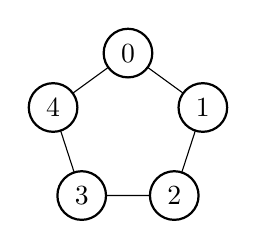
\begin{tikzpicture}
\tikzstyle{node}=[circle,draw,thick,fill=white]
\draw (90:1) node[node]{0}
-- (162:1) node[node]{4}
-- (234:1) node[node]{3}
-- (306:1) node[node]{2}
-- (378:1) node[node]{1}
-- cycle;
\end{tikzpicture}
\end{center}
$\forall i$ le noeud $i$ est pivot de $(i-1)\&(i+1)$ (modulo 5).

	\item On prend $G = $
\begin{center}  
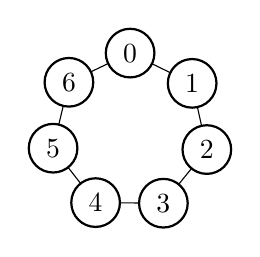
\begin{tikzpicture}
\tikzstyle{node}=[circle,draw,thick,fill=white]
\draw (90:1) node[node]{0}
-- (141:1) node[node]{6}
-- (192:1) node[node]{5}
-- (244:1) node[node]{4}
-- (295:1) node[node]{3}
-- (347:1) node[node]{2}
-- (398:1) node[node]{1}
-- cycle;
\end{tikzpicture}
\end{center}

$\forall i$ le noeud $i$ est pivot de : 
$(i-1) \& (i+1)$, $(i-1) \& (i+2)$ et $(i-2) \& (i+1)$ 
(modulo 7).
	\item Retirer le noeud pivot augmente la distance entre 2 personnes. Donc la probabilité que celles ci deviennent amies au temps $t+1$ diminue.

	\item On prouve d'abord que si un graphe n'a pas de cycle alors il possède au moins un noeud de degré 1.

Supposons que $G$ n'a pas de cycle et $V$ l'ensemble fini de ses noeuds.
Soit $x \in V$. On construit une séquence $P = (x_1, x_2, x_3, ...)$. Pour choisir $x_i (i>1)$, on prend un voisin de $x_{i-1}$ qiu n'a pas encore été choisi. Comme $V$ est fini, ce processus doit finir et on obtient $P= (x_1, x_2, x_3,...,x_k)$. 
Le noeud $k$ a un degré 1 car sinon il a un voisin $y\neq x_{k-1}$. Si $y \in P$ : Contradiction.
Si $y \notin P$, $x_k$ n'est pas la fin de la séquance : Contradiction.

On prouve ensuite que un noeud de degré un ne peu pas etre pivot.

Soit $x\in V$ tel que deg$(x)=1$.
Par hypothèse $x$ est pivot d'une paire $(y,z)$.
Donc il existe un chemin le plus court entre $y$ et $z$ qui passe bien par $x$.
Soit $w$ le seul voisin de $x$.
Mais alors il existe un chemin encore plus court : $(y, ..., w,...,z)$ qui ne passe pas par $x$.

% Insérer graphe 

\end{enumerate}
\subsection*{Exercice 2}
Soient $x, y$ et $z$ trois n\oe{}uds distincts. On dit que $x$ est un \emph{gardien} de $y$ et $z$ si tous les chemins entre $y$ et $z$ passent par $x$.
On dit qu'un n\oe{}ud $x$ est un \emph{gardien locale} s'il existent deux voisins de $x$ qui ne sont pas connect\'{e}s directement.
 
\begin{enumerate}
\item Donnez un exemple d'un graphe o\`{u} au moins la moiti\'{e} des n\oe{}uds sont
gardiens.
\item Donnez un exemple d'un graphe o\`{u} il n'y a pas de gardiens mais chaque n\oe{}ud est un gardien locale.
\item Quel est l'impacte sur un graphe de retirer un gardien?
\end{enumerate}

\subsubsection*{Solution}
\begin{enumerate}
	\item Les noeuds 1 et 2 sont gardien entre 0 et 3 

\begin{center}  
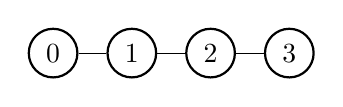
\begin{tikzpicture}
    \tikzstyle{node}=[circle,draw,thick,fill=white]
    \node[node] (0) at (0,0) {0};
    \node[node] (1) at (1,0) {1};
    \node[node] (2) at (2,0) {2};
    \node[node] (3) at (3,0) {3};

    \draw (0) -- (1);
    \draw (1) -- (2);
    \draw (2) -- (3);
\end{tikzpicture}
\end{center}

	\item  \hspace{1em}
	\vspace{1em}

\begin{center}  
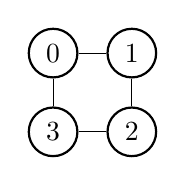
\begin{tikzpicture}
\tikzstyle{node}=[circle,draw,thick,fill=white]
    \node[node] (0) at (0,0) {0};
    \node[node] (1) at (1,0) {1};
    \node[node] (2) at (1,-1) {2};
    \node[node] (3) at (0,-1) {3};

    \draw (0) -- (1);
    \draw (1) -- (2);
    \draw (2) -- (3);
    \draw (3) -- (0);
\end{tikzpicture}
\end{center}

	\item Le graphe n'est plus connexe
\end{enumerate}

\subsection*{Exercice 3}

\begin{enumerate}
 \item Comment peut-on faire pour calculer efficacement les distances d'un n\oe{}uds a tout les autres?
 \item Un graphe est biparti si on peut s\'{e}parer les n\oe{}uds en deux ensembles $V_1$ et $V_2$ tells que
 $V_1 \cap V_2 = \emptyset$, $V_1 \cup V_2 = V$ et il n'y a pas d'ar\^{e}tes entre aucune paire de n\oe{}uds de $V_1$ et
 pas d'ar\^{e}tes entre aucune paire de n\oe{}uds de $V_2$. Soit $G$ un graphe connexe et $d_0(x)$ la distance du n\oe{}ud
 $0$ au n\oe{}ud $x$. Comment peut-on v\'{e}rifier que $G$ est bipartit a partir de $d_0$?
\end{enumerate}

\subsubsection*{Solution}
\begin{enumerate}

	\item On utilise l'algorithme BFS qui utilise une \texttt{Queue FIFO}
\begin{enumerate}
    \item Mettre le n\oe{}ud dans la Queue.
    \item Retirer le n\oe{}ud du début de la Queue pour l'examiner.
    \item Mettre tous les voisins non explorés dans la Queue.
    \item Si la file n'est pas vide reprendre à l'étape 2.
\end{enumerate}

Exemple : 

\begin{tabular}{lll}
    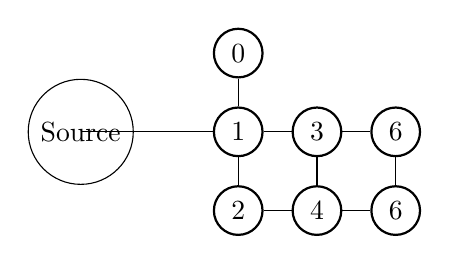
\begin{tikzpicture}
    \tikzstyle{node}=[circle,draw,thick,fill=white]
    \node[node] (2) at (0,0) {2};
    \node[node] (1) at (0,1) {1};
    \node[node] (0) at (0,2) {0};
    \node[node] (4) at (1,0) {4};
    \node[node] (3) at (1,1) {3};
    \node[node] (5) at (2,1) {6};
    \node[node] (6) at (2,0) {6};
    \node[] (S) at (-2,1) {Source};
    
    \draw (S) |- (1.west);
    \draw (0) -- (1);
    \draw (1) -- (2);
    \draw (3) -- (1);
    \draw (2) -- (4);
    \draw (4) -- (3);
    \draw (3) -- (5);
    \draw (6) -- (4);
    \draw (5) -- (6);
\end{tikzpicture}
&
  
&
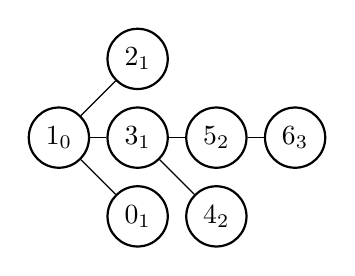
\begin{tikzpicture}
    \tikzstyle{node}=[circle,draw,thick,fill=white]
    \node[node] (1) at (0,1) {$1_{0}$};
    \node[node] (0) at (1,0) {$0_{1}$};
    \node[node] (3) at (1,1) {$3_{1}$};
    \node[node] (2) at (1,2) {$2_{1}$};
    \node[node] (5) at (2,1) {$5_{2}$};
    \node[node] (4) at (2,0) {$4_{2}$};
    \node[node] (6) at (3,1) {$6_{3}$};
    
    \draw (1) -- (0);
    \draw (1) -- (3);
    \draw (1) -- (2);
    \draw (3) -- (5);
    \draw (3) -- (4);
    \draw (5) -- (6);
\end{tikzpicture}
\end{tabular}

\item On vérifie qu'il n'existe pas d'arètes $(x,y)$ tel que $d_0(x)$ et $d_0(y)$ ont la meme parité

\end{enumerate}

% \vspace{0.5cm}
% 
% \subsection*{Exercice }
% Soient $x, y$ et $z$ trois n\oe{}uds distincts. On dit que $x$ est un \emph{gardien} de $y$ et $z$ si tous les chemins entre $y$ et $z$ passent par $x$.
% On dit qu'un n\oe{}ud $x$ est un \emph{gardien locale} s'il existent deux voisins de $x$ qui ne sont pas connect\'{e}s directement.
% 
% \begin{enumerate}
% \item Donnez un exemple d'un graphe o\`{u} au moins la moiti\'{e} des n\oe{}uds sont
% gardiens.
% \item Donnez un exemple d'un graphe o\`{u} il n'y a pas de gardiens mais chaque n\oe{}ud est un gardien locale.
% \end{enumerate}
% 

\subsection*{Exercice 4}
Le \emph{diam\`{e}tre} d'un graphe connexe est la distance maximum entre toutes les paires de n\oe{}uds. 
La \emph{distance moyenne} d'un graphe connexe c'est la moyenne des distances entre toutes les paires de n\oe{}uds. Formellement
$$
diam(G) = \max_{u, v} d(u, v)
$$
et
$$
l_G = \frac{1}{V (V - 1)} \sum_{u \neq v} d(u, v)
$$
o\'{u} $V$ est le nombre de n\oe{}uds de $G$.
\begin{enumerate}
\item Calculez le diam\`{e}tre et la distance moyenne du graphe $G_n$ suivant:
\begin{center}
\begin{tikzpicture}
\node[draw, circle] (A) at (0, 0) {0};
\node[draw, circle] (B) at (2, 0) {1};
\node[draw, circle] (C) at (4, 0) {2};
\node[draw, circle] (D) at (6, 0) {3};
\draw (A) -- (B) -- (C) -- (D);
\draw[dashed] (7, 0) circle (2);
\node at (9.5, 1) {$K_n$};
\draw (D) -- (7, 1);
\node at (7, 0.4) {$\vdots$};
\draw (D) -- (7, -0.5);
\draw (D) -- (7, -1);
\end{tikzpicture}
\end{center}
o\`{u} $K_n$ est le graphe complet avec $n$ n\oe{}uds. Par example, $G_4$ est le graphe:
\begin{center}
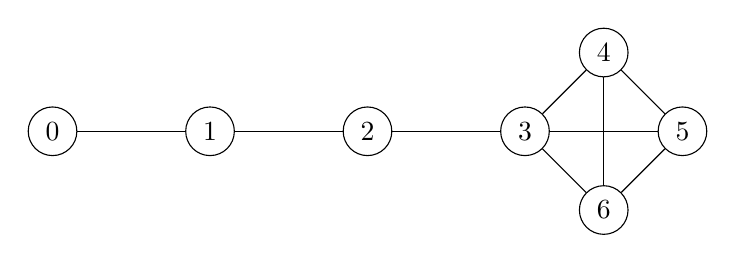
\begin{tikzpicture}
\node[draw, circle] (A) at (0, 0) {0};
\node[draw, circle] (B) at (2, 0) {1};
\node[draw, circle] (C) at (4, 0) {2};
\node[draw, circle] (D) at (6, 0) {3};
\node[draw, circle] (E) at (7, 1) {4};
\node[draw, circle] (F) at (8, 0) {5};
\node[draw, circle] (G) at (7, -1) {6};

\draw (A) -- (B) -- (C) -- (D);
\draw (D) -- (E);
\draw (D) -- (F);
\draw (D) -- (G);
\draw (E) -- (F);
\draw (E) -- (G);
\draw (G) -- (F);
\end{tikzpicture}
\end{center}


\item Montrez qu'il existe un graphe $G$ avec plus de $7$ n\oe{}uds tel que 
$$\frac{diam(G)}{l_G} = 2$$

\end{enumerate}


% \subsection*{Exercice }
% Calculez le coefficient regroupement de A et de B dans le graphe suivant:
% \begin{center}
% \begin{tikzpicture}
% \node[draw, circle] (A) at (0, 0)   {A};
% \node[draw, circle] (B) at (-2, 1)  {B};
% \node[draw, circle] (C) at (2, 1)   {C};
% \node[draw, circle] (D) at (2, -1)  {D};
% \node[draw, circle] (E) at (-2, -1) {E};
% \node[draw, circle] (F) at (-4, 0)  {F};
% \draw (A) -- (B);
% \draw (A) -- (C) -- (D);
% \draw (A) -- (D);
% \draw (A) -- (E) -- (B);
% \draw (B) -- (F) -- (E);
% \end{tikzpicture}
% \end{center}
% 
% 
% \vspace{0.5cm}

\subsubsection*{Solution}
\begin{enumerate}

	\item dim$(G) = 4$

Selon la table des distance:

\begin{tabular}{c|ccccc}
    &0&1&2&3& >3 \\
    \hline
    0 & 0& 1& 2& 3& 4\\
    1 & 1& 0&1& 2& 3\\
    2 & 2& 1& 0& 1&2\\
    3 & 1& 2& 3& 0&1\\
    >3 & 4& 3& 2& 1& 1 (0 si lui meme)\\
\end{tabular}

On peut calculer $\sum_{u\neq v} d(u,v)$.

\begin{align*}
    \sum_{u\neq v} d(u,v) =& 6 + 4(n-1)\\
    &+ 4 + 3(n-1)\\
    &+4+2(n-1)\\
    &+6+(n-1)\\
    &+(n-1)(10 + (n-2))\\
    =& 20 + (n-1)(4+3+2+1) + (n-1)(9 + (n-2))\\
    =& 20 + 10(n-1) + 9(n-1) + (n-1)^2\\
    =& 20 + 19(n-1) + (n-1)^2\\
    & \Rightarrow l_G (n) = \dfrac{n^2 + 17n + 2}{n^2 + 5n + 6}
\end{align*}


	\item $\dfrac{\text{diam}(G)}{l_G} = \dfrac{4}{l_G} =2$
\begin{align*}
    & \dfrac{4n^2 + 20n + 24}{n^2 + 17n + 2} = 2\\
    & \Rightarrow 4n^2 + 20n + 24 = 2n^2 + 34n + 4\\
    & \Rightarrow 2n^2 - 14n + 2\\
    & \Rightarrow n = 5\hspace{1em}\&\hspace{1em} n = 2\\
\end{align*}

Or $G$ doit comporter au moins 7 noeuds donc $G(5)$.

\end{enumerate}

\subsection*{Exercice 5}
On suppose qu'on est dans une communaut\'{e} ou les amiti\'{e}s sont repr\'{e}sent\'{e}es par un graphe $G$ connexe avec $n$ n\oe{}uds. 
Si chaque jour les amis des amis se rencontrent et deviennent amis, on s'interesse au nombre de jours $T(G)$ n\'{e}cessaires
pour que tout le monde deviennent ami, c'est-\`{a}-dire, pour le graphe deviennent $K_n$ (un graphe complet).
\begin{enumerate}
\item Supposons que $G = P_n$ (le chemin avec $n$ n\oe{}uds) et $T(P_n)$.
\item M\^{e}me question pour $G = C_n$ (le cycle avec $n$ n\oe{}uds).
\item Quel est la valeur de $T(G)$ en g\'{e}neral?
\end{enumerate}

\subsubsection*{Solution}
\begin{enumerate}

	\item Soit $A(i)$, les amis de $0$ au jour $i$.
\begin{align*}
    A(0) =& \{1 \} \\
    A(1) =& \{1,2 \}\\
    A(2) =& \{1,2,3,4 \}\\
    A(3) =& \{1,2,3,4,5,6,7,8, \}\\
    A(i) =& \{x+y | x,y \in A(i-1) \} \\
         =& \{1,2,3,..., 2^i \} \\
    T(P_n) =& \lceil \log_2 (n) \rceil
\end{align*}


	\item Le noeud le plus loin de $0$ dans un cycle de $n$ noeuds, est le noeud $\left\lfloor \dfrac{n}{2} \right\rfloor$
$$ T(C_n) = \left\lceil \log_2 \left(\left\lfloor \dfrac{n}{2} \right\rfloor \right) \right\rceil $$

	\item En général les noeuds à distance maximum prennent le plus de temps. Cette distance est le diamètre du graphe. Donc : 
$$ T(G) = \left\lceil \log_2 \left( \text{dim}(G) \right) \right\rceil $$


\end{enumerate}
% 
% \subsection*{Exercice }
% Calculez le coefficient de regroupement d'un n\oe{}ud de $C_n$, o\`{u} $n \geq 3$. Calculez le coefficient de regroupement de ce n\oe{}ud ap\`{e}s avoir ajout\'{e} les ar\^{e}tes entre les amis des amis dans le graphe. Commentez.
% 
% 
% 
% \subsection*{Exercice }
% \'{E}noncez la propri\'{e}t\'{e} de fermeture triadique forte. Est-ce que le graphe suivant poss\`{e}de cette propri\'{e}t\'{e}?
% 
% \begin{center}
% \begin{tikzpicture}
% \node[draw, circle] (A) at (0, 0) {A};
% \node[draw, circle] (B) at (2, 0) {B};
% \node[draw, circle] (C) at (0, -2) {C};
% \node[draw, circle] (D) at (-2, 0) {D};
% \node[draw, circle] (E) at (0, -4) {E};
% \node[draw, circle] (F) at (2, -2) {F};
% \node[draw, circle] (G) at (-2, -4) {G};
% \draw (G) -- (D) -- (A) -- (C) -- (F);
% \draw (C) -- (E);
% \draw[dashed] (G) -- (A) -- (B) -- (F) -- (E) -- (G);
% \draw[dashed] (D) -- (C);
% 
% \draw (4, -1) -- (5, -1) node[anchor = west] {lien fort};
% \draw[dashed] (4, -2) -- (5, -2) node[anchor = west] {lien faible};
% \end{tikzpicture}
% \end{center}
% 
% Supposons qu'un graphe poss\`{e}de la propri\'{e}t\'{e} de fermeture triadique forte. Si un lien faible devient fort, est-ce que cette propri\'{e}t\'{e} se maintien toujours? Et si un lien fort devient faible?
% 
% 


\section{}

% From TP4
\subsection{Exercise 1 (Authenticated encryption, or not; August Exam)}

Let $\Pi \define \langle \Gen, \Enc, \Dec\rangle$ be an authenticated encryption
scheme such that $\Enc$ encrypts messages of $n$ bits.
%
Do the following systems provide authenticated encryption?  For those
that do, briefly explain why.  For those that do not, present an
attack that breaks one of the security properties of an authenticated
encryption scheme.

\begin{enumerate}
	\item $\Pi' \define \langle \Gen, \Enc', \Dec'\rangle$ with
	$\Enc'_k(m) = (\Enc_k(m), \Enc_k(m \oplus (0^{n-1}\|1)))$ and
	$\Dec'_k(c_1, c_2) = \Dec_k(c_1)$ if
	$\Dec_k(c_1) \oplus \Dec_k(c_2) = 0^{n-1}\|1$ and $\bot$ otherwise.

	\item $\Pi' \define \langle \Gen, \Enc', \Dec'\rangle$ with
	$\Enc'_k(m) = (\Enc_k(m), \Mac_k(m))$ and $\Dec'_k(c_1, c_2) = \Dec_k(c_1)$

	if $\Vrfy_k(\Dec_k(c_1), c_2)=1$ and $\bot$ otherwise. Here, $\Mac$
	and $\Vrfy$ are deterministic algorithms that are part of a secure
	MAC scheme that is compatible with $\Gen$.
\end{enumerate}

\begin{solution}
	$\Pi \define \langle \text{Gen, Enc, Dec} \rangle$ is an authenticated encryption scheme (AE) if it is CCA-secure and unforgeable.
	\begin{enumerate}
		\item The system $\Pi'$ is not AE because it is \textbf{forgeable} and we can show it with this example. If the adversary A asks for the message $m$ ($m'$ corresponds to the message m with the last bit changed) to the oracle access, he will receive the cipher text $(c_1, c_2)$, where $c_1 = \Enc_k(m)$ and $c_2 = \Enc_k(m\xor 0^{n-1}||1) = \Enc_k(m')$.

		If $\A$ outputs the pair (m',$(c_2, c_1)$), this is a forgery.

		$\Dec_k'(c_2,c_1) = \Dec_k(c_2) = \Dec_k(\Enc_k(m')) = m' \neq \bot $ because $\Dec_k(c_2) \oplus \Dec_k(c_1) = m' \oplus m = m \oplus 0^{n-1}||1 \oplus m = 0^{n-1}||1 $.
		And $m'$ has not been requested before.

		Then we have EncForge$_{A, \Pi'}$(n) = 1  and Pr[EncForge$_{A, \Pi'}$(n)] = 1. $\Pi'$ is then forgeable and it is not an AE.

		With the same technique, an adversary can break the CCA-security of this scheme by querying two different messages $m_1$ and $m_2$, obtaining their encryption, sending \newline
		($m'_1,m'_2$) = ($m_1 \oplus 0^{n-1}||1, m_2 \oplus 0^{n-1}||1$) for the challenge, and compare the encryption of $m'_b$ with the two previously received ciphertexts.

		Note that this doesn't break CPA-security; indeed, the scheme is still CPA-secure.

		\item The sytem $\Pi'$ is not AE because it is not \textbf{CCA-secure} and we can show it because $Mac_k(m)$ does not assure any security (only authentication). So if We use as Mac:
		\[ \Mac_k(m) = m||\Mac'_k(m) \]
		It is a good mac but it is trivial to show that it is not CCA-Secure. $\Pi'$ is then not an AE.

		\strong{Stronger argument}:

		The adversary can send two different messages $m_0$ and $m_1$ to the encryption oracle to get $(\Enc_k(m_0), \Mac_k(m_0))$ and $(\Enc_k(m_1), \Mac_k(m_1))$.

		We then output the same $m_0$ and $m_1$, and receive $(\Enc_k(m_b), \Mac_k(m_b))$.

		As $\Pi$ is an athenticated encryption scheme, we know that $\Enc$ is probabilistic and secure.
		However, $\MAC$ is said to be deterministic, and this causes $\Mac_k(m_b)$ to be the same as one of the $\Mac_k(m_0)$, $\Mac_k(m_1)$ received earlier.
		We can thus just compare the tags, and output the corresponding $b'$.

		The probability of success is $\Pr[b'=b] = \Pr[\Mac_k(m0) \neq \Mac_k(m_1)]=1-\negl(n)$ which is clearly well above what it should be.
	\end{enumerate}
\end{solution}



\subsection{Exercise 2 (Derandomizing signatures)}

Let $S=(\Gen, \Sign, \Vrfy)$ be an EUF-CMA signature scheme defined over $(M, \Sigma)$, where the signing algorithm $\Sign$ is probabilistic.
In particular, algorithm $\Sign$ uses randomness chosen from a space $R$.
We let $\mathsf{S}(sk, m; r)$ denote the execution of algorithm $\mathsf{S}$ with randomness $r$.
Let $F$ be a secure PRF defined over $(K, M, R)$.
Show that the following signature scheme with deterministic signing $S'=(\Gen', \Sign', \Vrfy)$ is EUF-CMA:
\[ \mathsf{G}'(1^n) \define \left\{ (pk, sk) \pick \G(1^n), \qquad k \pick K, \qquad sk' \define (sk, k), \qquad \text{output } (pk, sk') \right\}; \]
\[ \Sign'((sk, k), m) \define \left\{ r \pick F_k(m), \qquad \sigma \pick \mathsf{S}(sk, m; r), \qquad \text{output } \sigma \right\}. \]

\emph{(Hint: Define $S''$ which is like $S'$ byt uses a perfect random function. Make a reduction of the security of $S''$ to the security of $S$, then build a PRF distinguisher based on a adversary against the signature. Finally, compute the link of the advantages of three relevant games.)}


\begin{solution}
	We will prove this in two steps.
	\begin{itemize}
		\item The first step defines $S''$ so that the PRF is replaced by a true random function.
		We will show that in this case, if $S$ is secure, then $S''$ is secure.
		\item The second step proves by reduction that if $S''$ is secure and $F$ is a secure PRF, then $S'$ is secure.
		The reduction proceeds by constructing an adversary $\A_{PRF}$ against the PRF, able to distinguish between the PRF and a random function, given an adversary $\A_{S'}$ against $S'$.
	\end{itemize}

	First, let's define $S''$.
	The only change is that
	\[ \Sign''((sk, k), m) \define \{ r \define f(m), \quad \sigma \define \mathsf{S}''(sk, m), \quad \text{output } \sigma \} \]
	where $\mathsf{S}''(sk, m) = \mathsf{S}(sk, m; f(m))$.

	If we have an adversary against $S''$, we can build an adversary against $S$, simply by relaying oracle calls to $\mathsf{S}_f''(sk, m)$ to our oracle $\mathsf{S}(sk, m; f(m))$.
	As $f$ is a random function, $S$ sees the same randomness as with an $r$, so nothing changes.
	The probabilities are exactly the same:
	\[ \Pr[\Sigforge_{S''}=1] = \Pr[\Sigforge_{S}=1] = \negl(n) \]
	for some $\negl$ negligible.

	Now, let's do the reduction from $F$ to $S'$.
	So, we have an adversary $\A_{S'}$ against $S'$, and we build an adversary against the PRF $\A_F$ as follows:
	\begin{enumerate}
		\item The oracle for the PRF problem $\O_F$ picks $k \pick \K$, kept secret.
		\item $\O_F$ picks $b \pick \bset$, kept secret.
		The oracle defines a challenge function $g=F_k$ if $b=1$, $g=f$ a random function if $b=0$.
		\item $\A_F$ runs $\Gen'$ to create a public key $pk$ and a secret key $sk'=(sk, k)$.
		It discards $k$ as it is not used by $\A_{S'}$ and is defined by $\O_F$.
		It keeps $sk$ secret and sends $pk$ to $\A_{S'}$.
		\item When $\A_{S'}$ asks for $\Sign'((sk, k), m)$, we ask the oracle for $w=g(m)$.
		$w=F_k(m)$ if $b=1$, or $w=f(m)$ with $f$ a random function, if $b=0$.
		We then run $\mathsf{S}(sk, m; r)$ and return the result to $\A_{S'}$.
		\item When $\A_{S'}$ outputs $(m, \sigma)$, its forgery, we outputs $b'=1$ iff $(m, sigma)$ is a valid forgery (we can verify it using $\Vrfy_{pk}$), $b'=0$ otherwise.
	\end{enumerate}
	If $b=0$, we're playing against a true random function, and so we're actually running the scheme $S''$.
	As $\A_{S'}$ is not designed to handle this scheme, its security is the same as the one of $S''$, which is the same as the one of $S$.

	If $b=1$, we're playing the true game for $\A_{S'}$, and so its advantage $\negl'(n)$ is active.

	Then, the difference in probabilities for the distinguishing is:
	\[ |\Pr[\A_F^{F_k}(n)] - \Pr[\A_F^{f}(n)]| = |\negl'(n) - \frac12 \negl(n)| \ge \negl'(n)-\negl(n) \]
	As this difference has to be negligible, as $F$ is a PRF, and $\negl$ is negligible, then $\negl'$ is negligible, and thus the scheme $S'$ is secure.
\end{solution}



\subsection{Exercise 3 (Jan 11 evaluation)}

\copypaste{9}{1}


\section{TP 11}
%\addcontentsline{toc}{section}{TP 11}

% \section*{Rappel}

% Structure du web:

% \begin{center}
% \includegraphics[scale = 0.5]{figs/web.png}
% \end{center}

% On repère trois composants principaux:
% \begin{itemize}
%  \item Un composant \textbf{in}, qui contient des liens hypertextes sortants.
%  \item Un composant fortement connecté principal, qui forme un \textbf{noyau} (SCC).
%  \item Un composant \textbf{out}, qui contient beaucoup de liens hypertextes entrants.
% \end{itemize}


% \newpage

% \section*{Exercices}


\subsection*{Exercice 1}
Considèrer de graphe avec 18 pages Web dans la Figure \ref{fig:webg}. Quels sont les noeuds qui font partie du noyau, les noeuds IN et les noeuds
OUT ? 

    \begin{figure}[h!]
    \begin{center}
    \includegraphics[scale = 0.3]{figs/graph.png}
    \end{center}
    \caption{Un graphe des pages web.}
    \label{fig:webg}
    \end{figure}

    \subsubsection*{Solution}

    \begin{center}
    \includegraphics[scale=0.5]{figs/TP11Q1.png}
    \end{center}


\subsection*{Exercice 2}
Pour le graphe de la Figure \ref{fig:webg}.
\begin{enumerate}
 \item Montrez une arête tel que si on l'ajoute ou on la retire, on augmente la taille du noyau.
 \item Montrez une arête tel que si on l'ajoute ou on la retire, on augmente la taille de IN.
 \item Montrez une arête tel que si on l'ajoute ou on la retire, on augmente la taille de OUT.
\end{enumerate}

    \subsubsection*{Solution}

    \begin{center}
    \includegraphics[scale=0.5]{figs/TP11Q2.png}
    \end{center}
    
    \begin{itemize}
        \item Le vert indique une arête à rajouter/retirer pour augmenter la taille du IN.
        \item Le rouge indique une arête à rajouter/retirer pour augmenter la taille du OUT.
        \item Le bleu indique une arête à rajouter pour augmenter la taille du SCC. Il n'est pas possible d'augmenter la taille du SCC en retirant une arête.
    \end{itemize}
    Il y a bien sûr d'autres possibilités que celles-là.


\subsection*{Exercice 3}
Décrivez un graphe tel qu'il existe une arête dont le retrait diminue la taille du noyeau d'au moins 1000 noeuds.

    \subsubsection*{Solution}
    Il faut pour cela un noyau qui possède un ensemble de 1000 noeuds ou plus qui n'est pas relié au IN ni au OUT et qui est relié au reste du noyau par seulement 2 arêtes : une entrante et une sortante.
    Supprimer l'arête qui va de cet ensemble au reste revient à rajouter l'ensemble au IN, tandis que supprimer l'autre arête revient à l'ajouter au OUT.


\subsection*{Exercice 4}
Décrivez un graphe tel qu'il existe une arête dont l'ajout diminue la taille de OUT d'au moins 1000 noueds.

    \subsubsection*{Solution}
    Il faut que le OUT possède une chaîne de 1000 noeuds ou plus et dont au moins un des noeuds de départ est directement lié au noyau.
    Il suffit de rajouter une arête au dernier noeud de cette chaîne pour qu'elle fasse partie intégrante du noyau, et donc pour diminuer la taille de OUT.

\subsection*{Exercice 5}
	\begin{enumerate}
	\item Calculez les valeurs de concentrateurs et d'autorités pour les pages dans le graphe présenté à la Figure \ref{fig:auth} après deux itérations.
	\item Quelles sont les valeurs une fois que la normalisation a été effectuée.
\end{enumerate}

\begin{figure}[!h]
	\centering
	\includegraphics[scale=0.4]{figs/auth-hub.png}
	\caption{graphe de page web}
	\label{fig:auth}
\end{figure}

    \subsubsection*{Algorithme de normalisation}
    
    \begin{itemize}
        \item \textbf{Init} :  $ \forall x \: auth(x) = hub(x) = 1 $
        \item \textbf{Steps}: \\
            $\forall x \: auth(x) = \sum_{y \in hub(x)} hub(y)  $ \\
            $\forall x \: hub(x) = \sum_{y \in auth(x)} auth(y)  $
        \item \textbf{Normalisation} : \\
            $ \forall x \: auth(x) = \frac{auth(x)}{\sum auth} $ \\
            $ \forall x \: hub(x) = \frac{hub(x)}{\sum hub} $
    \end{itemize}

    \subsubsection*{Solution}
    \begin{itemize}
        \item \textbf{Auth} : authorité : liens entrants
        \item \textbf{Conc} : concentrateur : liens sortants
    \end{itemize}

    \begin{center}
    	\begin{tabular}{c|ccccc}
    	     & A & B & C & D & E\\ \hline
    	Auth & 1 & 1 & 1 & 1 & 1\\
    	Conc & 1 & 1 & 1 & 1 & 1\\ \hline
    	Auth & 0 & 0 & 2 & 1 & 1\\
    	Conc & 1 & 3 & 0 & 0 & 0\\ \hline
    	Auth & 0 & 0 & 4 & 3 & 3\\
    	Conc & 2 & 4 & 0 & 0 & 0\\ \hline
    	\end{tabular}
    \end{center}
    
    Normalisation :
    \begin{center}
    	\begin{tabular}{c|ccccc}
    	     & A & B & C & D & E\\ \hline
    	Auth & 0 & 0 & 0.4 & 0.3 & 0.3\\
    	Conc & $\frac{1}{3}$ & $\frac{2}{3}$ & 0 & 0 & 0\\ \hline
    	\end{tabular}
    \end{center}
    
    
\subsection*{Exercice 6}
Calculez les valeurs de PageRank pour chaque page dans le graphe présenté à la Figure \ref{fig:pagerank} après deux itérations avec S = 1.


\begin{figure}[ht!]
	\centering
	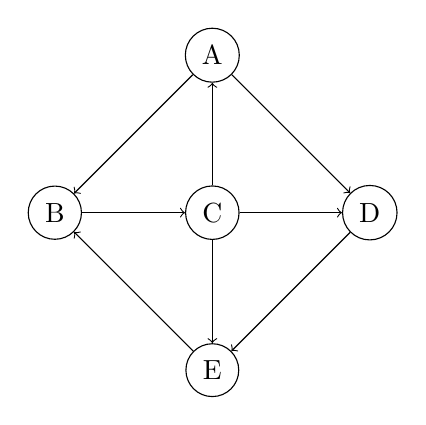
\begin{tikzpicture}[node distance=2cm]
		\tikzstyle{every node}=[draw=black,shape=circle]
		\node (c) at (0,0){C};
		\node[above of=c](a){A};
		\node[below of=c](e){E};
		\node[right of=c](d){D};
		\node[left of=c](b){B};

		\draw[->](a) -- (b);
		\draw[->](a) -- (d);
		\draw[->](b) -- (c);
		\draw[->](c) -- (a);
		\draw[->](c) -- (d);
		\draw[->](c) -- (e);
		\draw[->](d) -- (e);
		%\draw[->](d) -- (c);
		\draw[->](e) -- (b);
	\end{tikzpicture}
	\caption{graphe de page web}
	\label{fig:pagerank}
\end{figure}

    \subsubsection*{Solution}
    Règle de mise à jour : $Pr'(p) = S\ Pr(p) + (1-S) \frac{1}{n} = Pr(p)$.
    Seule la probabilité de suivre un lien à partir d'une page web entre en compte ici.\\
    À chaque itération k, on effectue les mises à jour suivantes :
    \begin{description}
        \item $Pr(A) = \frac{1}{3} Pr(C)$
        \item $Pr(B) = \frac{1}{2} Pr(A) + Pr(E)$
        \item $Pr(C) = Pr(B)$
        \item $Pr(D) = \frac{1}{2} Pr(A) + \frac{1}{3} Pr(C)$
        \item $Pr(E) = \frac{1}{3} Pr(C) + Pr(D)$
    \end{description}
    
    \begin{center}
        \begin{tabular}{c|ccccc}
        k & A & B & C & D & E\\ \hline 
    	0 & $\frac{1}{5}$ & $\frac{1}{5}$ & $\frac{1}{5}$ & $\frac{1}{5}$ & $\frac{1}{5}$\\ \\
    	1 & $\frac{1}{15}$ & $\frac{3}{10}$ & $\frac{1}{5}$ & $\frac{1}{6}$ & $\frac{4}{15}$\\ \\
    	2 & $\frac{1}{15}$ & $\frac{3}{10}$ & $\frac{3}{10}$ & $\frac{1}{10}$ & $\frac{7}{30}$\\
    	\end{tabular}
    \end{center}

\subsection*{Exercice 7}
Dans la Figure \ref{fig:equi}, les nombres à coté des noeuds représentent la valeur de PageRank de la page. Avec ce graphe, les valeurs de PageRank forment-elles un ensemble équilibré? Si oui pourquoi? Si non pourquoi?

\begin{figure}[ht!]
	\centering
	\includegraphics[scale=0.3]{figs/equi.png}
	\caption{graphe de page web}
	\label{fig:equi}
\end{figure}

    \subsubsection*{Solution}
    Il y a deux conditions à respecter pour que les valeurs de PageRank d'un graphe forment un ensemble équilibré :
    \begin{enumerate}
        \item La somme des valeurs doit valoir 1 : $\sum Pr(p_i) = 1$
        \item Une nouvelle itération doit donner les mêmes valeurs : $Pr'(p_i) = Pr(p_i) \ \forall p_i$\\
    \end{enumerate}
    
    Vérifions tout d'abord la première condition :
    $$ \sum Pr(p_i) = \frac{3}{10} + \frac{1}{10} + \frac{2}{10}  + \frac{1}{10}+  \frac{3}{10} = \frac{10}{10} = 1 $$

    Ensuite la seconde :
    \begin{description}
        \item $Pr'(A) = Pr(E) = \frac{3}{10} = Pr(A)$
        \item $Pr'(B) = \frac{1}{3} Pr(A) = \frac{1}{10} = Pr(B)$
        \item $Pr'(C) = \frac{1}{3} Pr(A) + \frac{1}{2} Pr(B) + \frac{1}{2} Pr(D) = \frac{2}{10} = Pr(C)$
        \item $Pr'(D) = \frac{1}{3} Pr(A) = \frac{1}{10} = Pr(D)$
        \item $Pr'(E) = \frac{1}{2} Pr(B) + Pr(C) + \frac{1}{2} Pr(D) = \frac{3}{10} = Pr(E)$\\
    \end{description}

    Nous pouvons donc conclure que nous cet ensemble de valeurs PageRank forme bien un ensemble équilibré.
    

\subsection*{Exercice 8}
		\begin{enumerate}
				\item Calculez les valeurs de PageRank pour chaque page dans le graphe présenté à la Figure \ref{fig:blackhole} après trois itérations avec S = 1.
				\item Que remarquez-vous? Selon vous comment vont évoluer les valeurs
						de PageRank pour un nombre d'itérations de plus en plus grand
				\item Calculez à nouveau les valeurs de PageRank pour chaque page mais pour 2 itérations avec S = 0.5.
		\end{enumerate}
		
    \begin{figure}[ht!]
	\centering
	
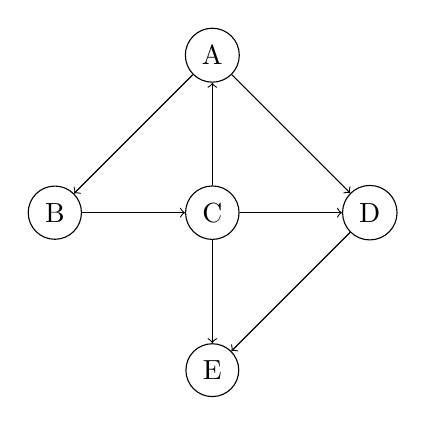
\begin{tikzpicture}[node distance=2cm]
	\tikzstyle{every node}=[draw=black,shape=circle]
	\node (c) at (0,0){C};
	\node[above of=c](a){A};
	\node[below of=c](e){E};
	\node[right of=c](d){D};
	\node[left of=c](b){B};

	\draw[->](a) -- (b);
	\draw[->](a) -- (d);
	\draw[->](b) -- (c);
	\draw[->](c) -- (a);
	\draw[->](c) -- (d);
	\draw[->](c) -- (e);
	\draw[->](d) -- (e);
	%\draw[->](d) -- (c);
	%\draw[->](e) -- (b);
\end{tikzpicture}
\caption{graphe de page web}
\label{fig:blackhole}
\end{figure}
		
    \subsubsection*{Solution}
    \begin{enumerate}
    
    \item Pour S=1, à chaque itération k, on effectue les mises à jour suivantes :
    \begin{description}
        \item $Pr(A) = \frac{1}{3} Pr(C)$
        \item $Pr(B) = \frac{1}{2} Pr(A)$
        \item $Pr(C) = Pr(B)$
        \item $Pr(D) = \frac{1}{2} Pr(A) + \frac{1}{3} Pr(C)$
        \item $Pr(E) = \frac{1}{3} Pr(C) + Pr(D) + Pr(E)$ \\
        \textit{(On ajoute $Pr(E)$ au calcul de E car c'est un noeud "cul-de-sac". Lors d'une itération, il faut prendre en compte le fait qu'une transition est bloquée au niveau de E et retombera donc vers E.)}
    \end{description}
    
    On obtient le résultat qui suit :
    \begin{center}
        \begin{tabular}{c|ccccc}
        k & A & B & C & D & E\\ \hline 
    	0 & $\frac{6}{30}$ & $\frac{6}{30}$ & $\frac{6}{30}$ & $\frac{6}{30}$ & $\frac{6}{30}$\\ \\
    	1 & $\frac{2}{30}$ & $\frac{3}{30}$ & $\frac{6}{30}$ & $\frac{5}{30}$ & $\frac{14}{30}$\\ \\
    	2 & $\frac{2}{30}$ & $\frac{1}{30}$ & $\frac{3}{30}$ & $\frac{3}{30}$ & $\frac{21}{30}$\\ \\
    	3 & $\frac{1}{30}$ & $\frac{1}{30}$ & $\frac{1}{30}$ & $\frac{2}{30}$ & $\frac{25}{30}$\\
    	\end{tabular}
    \end{center}
    
    \item On remarque qu'il y a une accumulation au niveau du noeud E.
    Sa valeur va tendre vers 1 alors que toutes les autres tendent vers 0.
    
    \item Pour S=0.5, à chaque itération k, on effectue les mises à jour suivantes :
    \begin{description}
        \item $Pr'(A) = \frac{1}{6} Pr(C) + \frac{1}{10}$
        \item $Pr'(B) = \frac{1}{4} Pr(A) + \frac{1}{10}$
        \item $Pr'(C) = \frac{1}{2} Pr(B) + \frac{1}{10}$
        \item $Pr'(D) = \frac{1}{4} Pr(A) + \frac{1}{6} Pr(C) + \frac{1}{10}$
        \item $Pr'(E) = \frac{1}{6} Pr(C) + \frac{1}{2} Pr(D) + \frac{1}{2} Pr(E) + \frac{1}{10}$
    \end{description}
    
    Le tableau résultant est :
    \begin{center}
        \begin{tabular}{c|ccccc}
        k & A & B & C & D & E\\ \hline 
    	0 & $\frac{6}{30}$ & $\frac{6}{30}$ & $\frac{6}{30}$ & $\frac{6}{30}$ & $\frac{6}{30}$\\ \\
    	1 & $\frac{4}{30}$ & $\frac{4.5}{30}$ & $\frac{6}{30}$ & $\frac{5.5}{30}$ & $\frac{10}{30}$\\ \\
    	2 & $\frac{4}{30}$ & $\frac{4}{30}$ & $\frac{5.25}{30}$ & $\frac{5}{30}$ & $\frac{11.75}{30}$\\
    	\end{tabular}
    \end{center}


\end{enumerate}

\end{document}
